\documentclass[11pt,a4paper]{article}
% Compile with XeLaTeX. Fonts reproduce the 2022 original: TeX Gyre Pagella text;
% Euler math letters (Latin and Greek, eulervm's zeur); newpx symbols and
% extension fonts; Latin Modern math operators and digits; bbold blackboard bold;
% Euler fraktur. The load order eulervm -> newpxmath -> Euler letters matches the
% set of fonts embedded in the original PDF.
\usepackage{amsmath,amssymb,amsthm,mathtools}
\usepackage{eulervm}
\usepackage{newpxmath}
\DeclareSymbolFont{letters}{U}{zeur}{m}{n}
\SetSymbolFont{letters}{bold}{U}{zeur}{b}{n}
% eulervm routes these to its own fonts; newpxmath does not re-declare them.
\DeclareMathSymbol{:}{\mathrel}{operators}{"3A}
\DeclareMathSymbol{\infty}{\mathord}{symbols}{"31}
\DeclareMathAlphabet{\mathfrak}{U}{euf}{m}{n}
\SetMathAlphabet{\mathfrak}{bold}{U}{euf}{b}{n}
\usepackage{bbold}
\usepackage[no-math]{fontspec}
\setmainfont{TeX Gyre Pagella}
\usepackage[margin=2.5cm]{geometry}
\usepackage{enumitem,booktabs,array}
\usepackage{tikz}
\usepackage{microtype}
\usepackage{xurl}
\usepackage[hidelinks]{hyperref}

\numberwithin{equation}{section}
\theoremstyle{plain}
\newtheorem{theorem}{Theorem}[section]
\newtheorem{lemma}[theorem]{Lemma}
\newtheorem{proposition}[theorem]{Proposition}
\newtheorem{corollary}[theorem]{Corollary}
\newtheorem*{theoremA}{Theorem A}
\newtheorem*{theoremB}{Theorem B}
\theoremstyle{definition}
\newtheorem{definition}[theorem]{Definition}
\newtheorem{construction}[theorem]{Construction}
\newtheorem{example}[theorem]{Example}
\newtheorem{question}{Question}
\theoremstyle{remark}
\newtheorem{remark}[theorem]{Remark}

\newcommand{\Q}{\mathbb{Q}}
\newcommand{\R}{\mathbb{R}}
\newcommand{\C}{\mathbb{C}}
\newcommand{\Z}{\mathbb{Z}}
\newcommand{\HT}{H^{*}_{T}}
\newcommand{\cL}{\mathcal{L}}
\newcommand{\cI}{\mathcal{I}}
\DeclareMathOperator{\Fl}{Fl}
\DeclareMathOperator{\Hess}{Hess}
\DeclareMathOperator{\Gr}{Gr}
\DeclareMathOperator{\ord}{ord}
\DeclareMathOperator{\rk}{rk}
\DeclareMathOperator{\cl}{cl}
\DeclareMathOperator{\Flats}{Flats}
\DeclareMathOperator{\Cl}{Cl}
\DeclareMathOperator{\GrH}{Gr}
\DeclareMathOperator{\St}{St}
\DeclareMathOperator{\cone}{cone}
\DeclareMathOperator{\trop}{trop}
\DeclareMathOperator{\Sym}{Sym}
\DeclareMathOperator{\diag}{diag}
\DeclareMathOperator{\Hom}{Hom}
\DeclareMathOperator{\OS}{OS}

\emergencystretch=3em
\hyphenation{Ay-zen-berg Che-re-pa-nov Bu-chs-ta-ber So-lo-ma-din equi-vari-antly}
\begin{document}

\begin{titlepage}
\centering
{\large Lomonosov Moscow State University\\
Faculty of Mechanics and Mathematics\\
Department of Higher Geometry and Topology\par}
\vspace{3cm}
{\large Diploma thesis (Specialist degree)\par}
\vspace{1.2cm}
{\LARGE\bfseries Invariants of matroids\\[4pt] defined by torus actions\par}
\vspace{3cm}
\begin{flushright}
\begin{tabular}{r}
Author: David A.~Mikheev, group 605\\[10pt]
Scientific advisor:\\
Corresponding Member of the RAS, Professor\\
Victor M.~Buchstaber
\end{tabular}
\end{flushright}
\vfill
{\large Moscow, 2022\par}
\vspace{4pt}
{\normalsize Revised English edition, 2026\par}
\end{titlepage}

\begin{abstract}
We study the combinatorics of the face poset $S(X)$ of an action of a compact torus $T$ of positive complexity on a manifold~$X$. The aim is to investigate connections between known constructions in matroid theory, toric geometry and toric topology. We prove that the local equivariant cohomology $\HT(X,X\setminus pt)$ at a fixed point $pt$, viewed through restriction to $pt$ as an ideal of $\HT(pt)$, is the principal ideal generated by the product of the tangent weights at $pt$; it therefore determines the linear matroid of weights at $pt$, multiplicities included, and hence the geometric lattice $S(X)_{\geqslant pt}$ of faces whose closures contain $pt$. As a counterpoint, we show that this local data is far from determining the global equivariant cohomology: we exhibit two connected regular semisimple Hessenberg varieties in $\Fl(\C^5)$, with torus actions of complexity one, whose local weight matroids are isomorphic at every fixed point --- so that the Chow rings and Orlik--Solomon algebras of these matroids coincide --- while their equivariant cohomology modules are not isomorphic.
\end{abstract}

\paragraph{About this edition.}
This is an English translation and revision of the Russian text of 2022. Errors identified in an audit of the original have been corrected; the counterexample announced but not proved in the original is proved in Section~\ref{sec:counterexample}; the descriptions of face posets of Hessenberg varieties and of the cycle cluster-permutohedra have been corrected and attributed to their sources; and the references have been updated. A complete list of changes, each tied to an audit item, is kept in \texttt{docs/thesis-v2/CHANGES.md} of the repository \url{https://github.com/davidmiheev/matroid_toric}, which also contains the programs behind every computation cited here (Appendix~\ref{app:computations}).

\newpage
\tableofcontents
\newpage

%======================================================================
\section{Introduction}
%======================================================================

The study of spaces with torus actions of complexity zero lies at the foundation of toric geometry and toric topology. The foundations of toric topology and its applications are presented in the monograph of V.~M.~Buchstaber and T.~E.~Panov~\cite{BP15}. Buchstaber and S.~Terzić posed the problem of extending the methods of toric topology to actions of positive complexity. They developed such methods and demonstrated them on the Grassmann manifold $\Gr(2,4)$, with a torus action of complexity one, and on $\Gr(2,5)$, with complexity two~\cite{BT19a,BT19b}. The original object of their theory is a smooth $2n$-dimensional manifold with an effective action of a compact $k$-dimensional torus and a discrete set of fixed points~\cite{BT19b}. They developed an axiomatics of such manifolds which does not assume a priori that the action of the compact torus extends to an action of the algebraic torus; their main results, however, concern situations in which it does. In the works of A.~Ayzenberg, M.~Masuda and their coauthors~\cite{AC22,AMS23,AB24}, an approach to such actions was developed whose central object is the \emph{face poset} of the action.

Throughout, a torus action on $X$ means an effective action of a compact torus on a closed smooth manifold $X$ with a nonempty finite set of fixed points. This work belongs to the framework of Ayzenberg and Masuda. Its focus is the connection between the face poset $S(X)$ of a torus action and matroid theory, more precisely, between $S(X)$ and the matroids, described by their geometric lattices of flats, that are attached to the fixed points of the action.

The main directions of this work are:
\begin{itemize}[nosep]
\item the combinatorics of the face poset $S(X)$ of torus actions of positive complexity;
\item connections between constructions in matroid theory, toric topology and toric geometry;
\item the relation between the local equivariant cohomology of a torus action and its face poset.
\end{itemize}

The face poset $S(X)$ is locally geometric (Theorem~\ref{thm:AC}, due to Ayzenberg and Cherepanov~\cite{AC22}): to each fixed point $p$ one associates the linear matroid of tangent weights at $p$, whose lattice of flats is the subposet $S(X)_{\geqslant p}$ of faces whose closure contains $p$. The posets $S(X)_{\geqslant p}$ thus cover $S(X)$. Our main results are the following.

\begin{theoremA}[Theorem~\ref{thm:main}]
Let a torus $T$ act on $X$ with arbitrary complexity, and let $pt$ be a fixed point. Restriction to $pt$ identifies the local equivariant cohomology $\HT(X,X\setminus pt)$ with the principal ideal of $\HT(pt)=H^*(BT;\Q)$ generated by the product of the tangent weights at $pt$. This ideal determines the multiset of tangent weights up to nonzero scalars; hence it determines the linear matroid of weights and the geometric lattice $S(X)_{\geqslant pt}$.
\end{theoremA}

\begin{theoremB}[Theorem~\ref{thm:counterexample}]
The equivariant cohomology of a torus manifold is not determined by the linear matroids of weights at its fixed points, and in particular not by the Chow rings and Orlik--Solomon algebras of these matroids. There exist two connected regular semisimple Hessenberg varieties $X_1,X_2\subset\Fl(\C^5)$, with actions of complexity one of the same torus, whose weight matroids are isomorphic at all fixed points, while $\HT(X_1)\not\cong\HT(X_2)$.
\end{theoremB}

We also describe the posets $S(X)$ for important classes of manifolds with torus actions of positive complexity --- full and partial flag varieties, regular semisimple Hessenberg varieties and their partial analogues --- following Ayzenberg and Buchstaber~\cite{AB21,AB24}.

Let us describe the main notions and methods and give a brief survey of the related literature. Gelfand and Serganova~\cite{GS87} (see also~\cite{GGMS87}) studied matroids in the context of torus strata on Grassmannians. In the present work matroids appear in a more general context. The main emphasis is on GKM theory~\cite{GKM98}; we use methods of matroid theory, representation theory and toric topology.

Matroids were introduced by H.~Whitney~\cite{Whi35}, and matroid theory has since developed extensively; its foundations are presented in the book of J.~Oxley~\cite{Oxl11}, from which we take several basic definitions. Orlik--Solomon algebras~\cite{OT92} appear in toric geometry and toric topology, and Chow rings of algebraic varieties are used in the parametric toric topology developed by Buchstaber and Terzić. We include a review of Chow rings defined for matroids and examine whether the equivariant cohomology of a torus action is determined by the Chow rings and Orlik--Solomon algebras of its local weight matroids; Theorem~B shows that it is not. The interest in Chow rings of matroids comes from recent work, notably of K.~Adiprasito, J.~Huh and E.~Katz~\cite{AHK18} (see also~\cite{Huh14}), who established for Chow rings of matroids a number of properties that are usually characteristic of rings attached to geometric objects. Also of interest is the work of Adiprasito~\cite{Adi18}, whose results yield the $g$-theorem for rational homology spheres. We also touch upon some aspects of tropical geometry; a good introduction is the book of D.~Maclagan and B.~Sturmfels~\cite{MS15}.

\paragraph{Contents of the work.}
\begin{itemize}[nosep]
\item Section~\ref{sec:matroids} contains the definitions and facts about matroids and posets used in the work.
\item Section~\ref{sec:equivariant} is a brief introduction to equivariant cohomology, with an emphasis on torus actions, and contains the examples of spaces with torus actions used later.
\item Section~\ref{sec:GKM} contains the main results: the meaning of local equivariant cohomology in terms of the combinatorial objects studied here (Section~\ref{sec:local}), the face posets of the examples (Section~\ref{sec:faces}), and the counterexample (Section~\ref{sec:counterexample}).
\item Section~\ref{sec:tropical} describes some related facts of tropical geometry.
\item Appendix~\ref{app:computations} describes the computations.
\end{itemize}

\paragraph{Conventions.}
All (co)homology has coefficients in $\Q$ unless stated otherwise. For a compact torus $T=T^k$ we identify $H^*(BT;\Q)=\Sym(\mathfrak t^*_\Q)\cong\Q[t_1,\dots,t_k]$ with $\deg t_i=2$, and $H^2(BT;\Q)\cong\Hom(T,S^1)\otimes\Q$.

%======================================================================
\section{Matroids and posets}\label{sec:matroids}
%======================================================================

We begin with the definitions and constructions used in what follows. This section concerns matroids and related notions, i.e.\ the combinatorial side of the work.

\subsection{Basic definitions and constructions}

There are several cryptomorphic definitions of a matroid; we use independent sets.

\begin{definition}[Matroid]\label{def:matroid}
A \emph{matroid} is a pair $M=(E,\cI)$, where $E$ is a finite set and $\cI$ is a family of subsets of $E$ such that
\begin{itemize}[nosep]
\item $\varnothing\in\cI$;
\item if $A\in\cI$ and $A'\subseteq A$, then $A'\in\cI$;
\item if $A,B\in\cI$ and $|A|>|B|$, then there is $x\in A\setminus B$ with $B\cup\{x\}\in\cI$.
\end{itemize}
The elements of $\cI$ are called \emph{independent sets}.
\end{definition}

\begin{definition}[Rank]
The \emph{rank} $r_M(S)$ of a subset $S\subseteq E$ is the cardinality of a maximal independent subset of $S$. The rank of $M$ is $r(M)=r_M(E)$.
\end{definition}

\begin{definition}[Flat]
A \emph{flat} of $M$ is a subset $F\subseteq E$ such that adding any element of $E\setminus F$ increases the rank. The \emph{closure} $\cl(A)$ of $A\subseteq E$ is the smallest flat containing~$A$. An element $e$ is a \emph{loop} if $\{e\}\notin\cI$; $M$ is \emph{loopless} if it has no loops.
\end{definition}

\begin{example}[Uniform matroid]
The \emph{uniform matroid} $U_{r,n}$ is the matroid on $[n]=\{1,\dots,n\}$ whose independent sets are all subsets of cardinality at most $r$.
\end{example}

\begin{example}[Graphic matroid]\label{ex:graphic}
Let $G$ be a graph. The \emph{graphic} (cycle) matroid $M(G)$ has the set of edges of $G$ as ground set, and its independent sets are the edge sets of forests in~$G$.
\end{example}

\begin{definition}
A \emph{poset} (partially ordered set) is a set with a partial order. An element $y$ \emph{covers} $x$ if $y>x$ and there is no $z$ with $y>z>x$.
\end{definition}

Posets are visualized by Hasse diagrams: elements are vertices, and an edge goes up from $x$ to $y$ whenever $y$ covers $x$.

\begin{construction}[Order complex]
The \emph{order complex} $\ord(S)$ of a poset $S$ is the simplicial complex on the vertex set $S$ whose simplices are the chains (totally ordered subsets) of $S$. A chain of $k$ elements is a $(k-1)$-simplex. The order complex is a flag complex.
\end{construction}

\begin{definition}
For $x\in S$ we set $S_{\geqslant x}=\{t\in S\mid t\geqslant x\}$, and similarly $S_{\leqslant x}$, $S_{>x}$, $S_{<x}$. A \emph{least element} $\hat0$ satisfies $\hat0\leqslant t$ for all $t$; a \emph{greatest element} $\hat1$ satisfies $t\leqslant\hat1$ for all $t$.
\end{definition}

\begin{definition}[Graded poset]
A \emph{rank function} on a finite poset $S$ is a function $r\colon S\to\Z_{\geqslant0}$ such that $r(x)=0$ for minimal $x$ and $r(y)=r(x)+1$ whenever $y$ covers $x$. A poset admitting a rank function is \emph{graded}.
\end{definition}

Not every poset is graded: a poset with $\hat0$ and $\hat1$ is not graded if it has maximal chains from $\hat0$ to $\hat1$ of different lengths. A \emph{lattice} is a poset in which any two elements $x,y$ have a least upper bound $x\vee y$ (join) and a greatest lower bound $x\wedge y$ (meet).

\begin{definition}[Geometric lattice]
A \emph{geometric lattice} is a finite graded lattice such that
\begin{itemize}[nosep]
\item every element is a join of atoms (the elements covering $\hat0$);
\item $r(x)+r(y)\geqslant r(x\vee y)+r(x\wedge y)$ for all $x,y$ (semimodularity).
\end{itemize}
\end{definition}

\begin{definition}[Lattice of flats]
The flats of a matroid $M$, ordered by inclusion, form a geometric lattice $\cL_M$, the \emph{lattice of flats}. Its least element is $\cl(\varnothing)$ and its greatest element is $E$; the rank of a flat in $\cL_M$ is its rank in $M$. Conversely, every geometric lattice is the lattice of flats of a unique simple matroid~\cite{Oxl11}.
\end{definition}

\begin{figure}[ht]
\centering
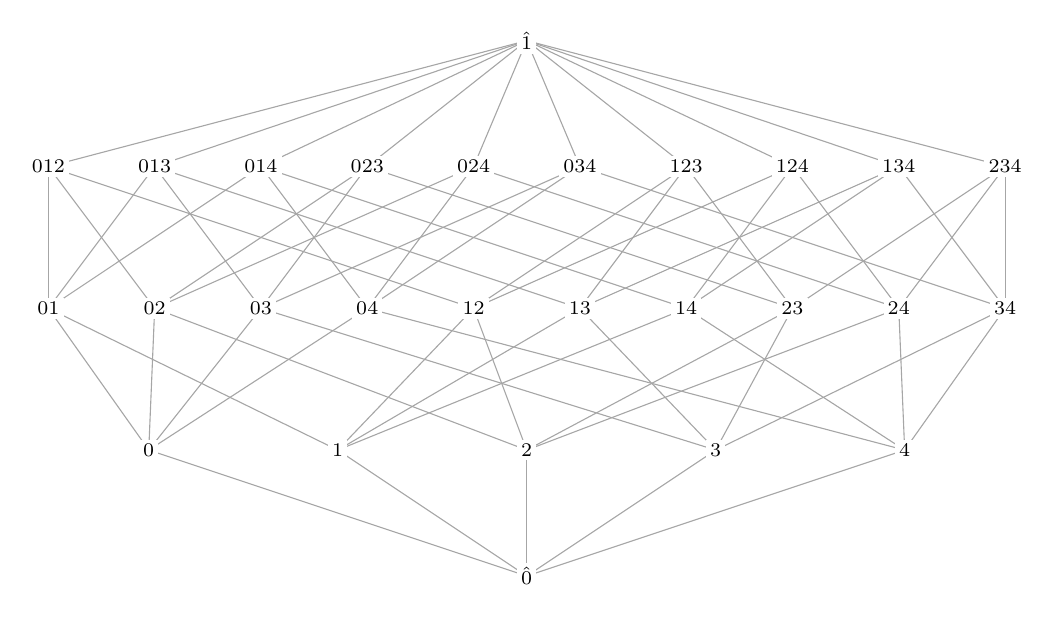
\begin{tikzpicture}[x=1cm,y=1cm,every node/.style={font=\scriptsize,inner sep=1.5pt,fill=white}]
\coordinate (bot) at (0.000,0.000);
\coordinate (s0) at (-4.800,1.600);
\coordinate (s1) at (-2.400,1.600);
\coordinate (s2) at (0.000,1.600);
\coordinate (s3) at (2.400,1.600);
\coordinate (s4) at (4.800,1.600);
\coordinate (s01) at (-6.075,3.400);
\coordinate (s02) at (-4.725,3.400);
\coordinate (s03) at (-3.375,3.400);
\coordinate (s04) at (-2.025,3.400);
\coordinate (s12) at (-0.675,3.400);
\coordinate (s13) at (0.675,3.400);
\coordinate (s14) at (2.025,3.400);
\coordinate (s23) at (3.375,3.400);
\coordinate (s24) at (4.725,3.400);
\coordinate (s34) at (6.075,3.400);
\coordinate (s012) at (-6.075,5.200);
\coordinate (s013) at (-4.725,5.200);
\coordinate (s014) at (-3.375,5.200);
\coordinate (s023) at (-2.025,5.200);
\coordinate (s024) at (-0.675,5.200);
\coordinate (s034) at (0.675,5.200);
\coordinate (s123) at (2.025,5.200);
\coordinate (s124) at (3.375,5.200);
\coordinate (s134) at (4.725,5.200);
\coordinate (s234) at (6.075,5.200);
\coordinate (top) at (0.000,6.800);
\draw[gray!70] (bot) -- (s0);
\draw[gray!70] (bot) -- (s1);
\draw[gray!70] (bot) -- (s2);
\draw[gray!70] (bot) -- (s3);
\draw[gray!70] (bot) -- (s4);
\draw[gray!70] (s0) -- (s01);
\draw[gray!70] (s0) -- (s02);
\draw[gray!70] (s0) -- (s03);
\draw[gray!70] (s0) -- (s04);
\draw[gray!70] (s1) -- (s01);
\draw[gray!70] (s1) -- (s12);
\draw[gray!70] (s1) -- (s13);
\draw[gray!70] (s1) -- (s14);
\draw[gray!70] (s2) -- (s02);
\draw[gray!70] (s2) -- (s12);
\draw[gray!70] (s2) -- (s23);
\draw[gray!70] (s2) -- (s24);
\draw[gray!70] (s3) -- (s03);
\draw[gray!70] (s3) -- (s13);
\draw[gray!70] (s3) -- (s23);
\draw[gray!70] (s3) -- (s34);
\draw[gray!70] (s4) -- (s04);
\draw[gray!70] (s4) -- (s14);
\draw[gray!70] (s4) -- (s24);
\draw[gray!70] (s4) -- (s34);
\draw[gray!70] (s01) -- (s012);
\draw[gray!70] (s01) -- (s013);
\draw[gray!70] (s01) -- (s014);
\draw[gray!70] (s02) -- (s012);
\draw[gray!70] (s02) -- (s023);
\draw[gray!70] (s02) -- (s024);
\draw[gray!70] (s03) -- (s013);
\draw[gray!70] (s03) -- (s023);
\draw[gray!70] (s03) -- (s034);
\draw[gray!70] (s04) -- (s014);
\draw[gray!70] (s04) -- (s024);
\draw[gray!70] (s04) -- (s034);
\draw[gray!70] (s12) -- (s012);
\draw[gray!70] (s12) -- (s123);
\draw[gray!70] (s12) -- (s124);
\draw[gray!70] (s13) -- (s013);
\draw[gray!70] (s13) -- (s123);
\draw[gray!70] (s13) -- (s134);
\draw[gray!70] (s14) -- (s014);
\draw[gray!70] (s14) -- (s124);
\draw[gray!70] (s14) -- (s134);
\draw[gray!70] (s23) -- (s023);
\draw[gray!70] (s23) -- (s123);
\draw[gray!70] (s23) -- (s234);
\draw[gray!70] (s24) -- (s024);
\draw[gray!70] (s24) -- (s124);
\draw[gray!70] (s24) -- (s234);
\draw[gray!70] (s34) -- (s034);
\draw[gray!70] (s34) -- (s134);
\draw[gray!70] (s34) -- (s234);
\draw[gray!70] (s012) -- (top);
\draw[gray!70] (s013) -- (top);
\draw[gray!70] (s014) -- (top);
\draw[gray!70] (s023) -- (top);
\draw[gray!70] (s024) -- (top);
\draw[gray!70] (s034) -- (top);
\draw[gray!70] (s123) -- (top);
\draw[gray!70] (s124) -- (top);
\draw[gray!70] (s134) -- (top);
\draw[gray!70] (s234) -- (top);
\node at (bot) {$\hat 0$};
\node at (s0) {$0$};
\node at (s1) {$1$};
\node at (s2) {$2$};
\node at (s3) {$3$};
\node at (s4) {$4$};
\node at (s01) {$01$};
\node at (s02) {$02$};
\node at (s03) {$03$};
\node at (s04) {$04$};
\node at (s12) {$12$};
\node at (s13) {$13$};
\node at (s14) {$14$};
\node at (s23) {$23$};
\node at (s24) {$24$};
\node at (s34) {$34$};
\node at (s012) {$012$};
\node at (s013) {$013$};
\node at (s014) {$014$};
\node at (s023) {$023$};
\node at (s024) {$024$};
\node at (s034) {$034$};
\node at (s123) {$123$};
\node at (s124) {$124$};
\node at (s134) {$134$};
\node at (s234) {$234$};
\node at (top) {$\hat 1$};
\end{tikzpicture}

\caption{The lattice of flats of $U_{4,5}$: all subsets of $\{0,\dots,4\}$ of size at most $3$, together with $\hat1=E$.}
\label{fig:u45}
\end{figure}

\begin{definition}[Möbius function]
The \emph{Möbius function} of a finite poset is defined inductively by
\[
\mu(x,y)=\begin{cases}1,& x=y,\\ -\sum_{x\leqslant z<y}\mu(x,z),& x<y,\\ 0,&\text{otherwise.}\end{cases}
\]
\end{definition}

The Möbius function of a geometric lattice has good properties. For instance, Rota's sign theorem states that $(-1)^{r(B)-r(A)}\mu(A,B)>0$ for all $A\leqslant B$ in a geometric lattice~\cite{Bjo92}.

\begin{definition}[Characteristic polynomial]
The \emph{characteristic polynomial} of a loopless matroid $M$ is
\[
\chi_M(t)=\sum_{F\in\cL_M}\mu(\hat0,F)\,t^{\,r(E)-r(F)}.
\]
\end{definition}

The sum over the lattice of flats can be rewritten as a sum over all subsets of the ground set.

\begin{proposition}[Whitney]\label{prop:whitney}
For a loopless matroid $M$ on $E$,
\[
\chi_M(t)=\sum_{A\subseteq E}(-1)^{|A|}\,t^{\,r(E)-r(A)}.
\]
\end{proposition}
\begin{proof}
Grouping subsets by their closure and using $r(A)=r(\cl A)$, the right-hand side equals $\sum_{F\in\cL_M}g(F)\,t^{r(E)-r(F)}$ with $g(F)=\sum_{A:\,\cl A=F}(-1)^{|A|}$. For every flat $F$ we have $\sum_{G\leqslant F}g(G)=\sum_{A\subseteq F}(-1)^{|A|}$, which is $1$ if $F=\varnothing$ and $0$ otherwise. Since $M$ is loopless, $\hat0=\varnothing$, so this says $\sum_{G\leqslant F}g(G)=\delta_{\hat0,F}$, and Möbius inversion gives $g(F)=\mu(\hat0,F)$.
\end{proof}

\begin{definition}[Pure complex]
A simplicial complex is \emph{pure} if all its maximal simplices have the same dimension.
\end{definition}

As noted above, the order complex is a flag complex; for a graded poset it is moreover pure. For a geometric lattice $\cL$ of rank $r$, the maximal simplices of $\ord(\cL\setminus\{\hat0,\hat1\})$ are the maximal chains of proper elements, which have $r-1$ elements, so this complex is pure of dimension $r-2$. Pure complexes play an important role in combinatorial topology.

\begin{construction}[Shellable complexes]
A pure complex is \emph{shellable} if its maximal simplices can be ordered so that the intersection of each of them with the union of the preceding ones is a nonempty union of maximal proper faces of it (that is, a pure complex of dimension one less).
\end{construction}

The order complex of a geometric lattice itself is a cone, hence contractible. The interesting object is the order complex of $\cL\setminus\{\hat0,\hat1\}$.

\begin{proposition}[\cite{Bjo92}]
For a geometric lattice $\cL$, the complex $\ord(\cL\setminus\{\hat0,\hat1\})$ is shellable. A shellable complex is homotopy equivalent to a wedge of spheres of its dimension.
\end{proposition}

\begin{proposition}\label{prop:euler}
Let $\cL$ be a geometric lattice of rank $r\geqslant2$. Then $\ord(\cL\setminus\{\hat0,\hat1\})$ is homotopy equivalent to a wedge of $|\mu(\hat0,\hat1)|$ spheres of dimension $r-2$, and its reduced Euler characteristic is
\[
\tilde\chi\bigl(\ord(\cL\setminus\{\hat0,\hat1\})\bigr)=\mu(\hat0,\hat1)=(-1)^r\,|\mu(\hat0,\hat1)|.
\]
\end{proposition}
\begin{proof}
By the previous proposition the complex is a wedge of, say, $m$ spheres of dimension $r-2$, so $\tilde\chi=(-1)^{r-2}m=(-1)^rm$. By P.~Hall's theorem, $\tilde\chi(\ord(P\setminus\{\hat0,\hat1\}))=\mu_P(\hat0,\hat1)$ for every finite bounded poset $P$ (see~\cite{Bjo92}). Hence $(-1)^rm=\mu(\hat0,\hat1)$, and Rota's sign theorem gives $m=|\mu(\hat0,\hat1)|$.
\end{proof}

\begin{remark}
The sign matters. For the Boolean lattice of rank $3$ one has $\mu(\hat0,\hat1)=-1$, and the proper part is a hexagon, a circle, whose unreduced Euler characteristic is $0=1+\mu(\hat0,\hat1)$.
\end{remark}

We will also use the following class of graphs.

\begin{construction}[Indifference graphs]\label{con:indifference}
An \emph{indifference graph} (unit interval graph) is a graph whose vertices are points of the real line, two points being adjacent if their distance is at most $1$. For a Hessenberg function $h$ (Example~\ref{ex:hessenberg}), let $\Gamma_h$ be the graph on $[n]$ with edges $\{j,i\}$ for $j<i\leqslant h(j)$. The graphs $\Gamma_h$ are, up to isomorphism, exactly the indifference graphs; see~\cite[Rem.~3.1]{AB21}. The path graph on $n$ vertices is $\Gamma_h$ for $h=(2,3,\dots,n,n)$.
\end{construction}

The following notions are used only briefly, but they are important.

\begin{definition}
A \emph{polyhedral cone} in $\R^n$ is a set $\cone(v_1,\dots,v_r)=\{\sum_{j=1}^r\lambda_jv_j\mid\lambda_j\geqslant0\}$. A \emph{polyhedral fan} $\Sigma$ is a collection of cones such that every face of a cone in $\Sigma$ is in $\Sigma$, and the intersection of two cones of $\Sigma$ is a face of each. A \emph{polyhedral complex} is a collection of polyhedra with the same two properties, where the intersection of two polyhedra is either empty or a common face.
\end{definition}

\begin{definition}[Bergman fan]
Let $M$ be a loopless matroid on $E$. For $F\subseteq E$ put $e_F=\sum_{i\in F}e_i\in\R^E/\R e_E$. The (fine subdivision of the) \emph{Bergman fan} $\Sigma_M$ is the fan of cones $\cone(e_{F_1},\dots,e_{F_k})$, where $F_1\subsetneq\dots\subsetneq F_k$ runs over all chains of nonempty proper flats of $M$~\cite{AK06,FY04}. (Depending on the min/max convention in tropical geometry, $-e_F$ is used instead of $e_F$.)
\end{definition}

The following ring is an analogue of the Stanley--Reisner ring of a simplicial complex, or of the cohomology ring of a manifold, defined for an arbitrary matroid.

\begin{definition}[Chow ring of a matroid~{\cite[Def.~1.3]{AHK18}}]\label{def:chow}
Let $M$ be a loopless matroid on $E$ and $k$ a field, and let $S_M=k[x_F\mid F\text{ a nonempty proper flat of }M]$. The \emph{Chow ring} of $M$ is $A^*(M)=S_M/(I_M+J_M)$, where $I_M$ is generated by the monomials $x_{F_1}x_{F_2}$ for incomparable nonempty proper flats $F_1,F_2$, and $J_M$ is generated by the linear forms
\[
\sum_{F\ni i_1}x_F-\sum_{F\ni i_2}x_F,\qquad i_1\neq i_2\in E.
\]
\end{definition}

The ring $A^*(M)$ is graded, $A^*(M)=\bigoplus_{q=0}^{r(M)-1}A^q(M)$, and $A^{r(M)-1}(M)\cong k$ via the degree map sending $x_{F_1}\cdots x_{F_{r(M)-1}}$ to $1$ for every maximal flag of nonempty proper flats~\cite{AHK18}. By~\cite{FY04} (see~\cite[§1]{AHK18}), $A^*(M)$ is the Chow ring of the smooth, noncomplete toric variety $X(\Sigma_M)$ of the Bergman fan.

\begin{definition}[Orlik--Solomon algebra~\cite{OT92}]
Let $M$ be a loopless matroid on $E$ and $\Lambda$ the exterior algebra over $k$ with generators $e_i$, $i\in E$. Let $\partial$ be the derivation of degree $-1$ with $\partial e_i=1$. The \emph{Orlik--Solomon algebra} is $\OS(M)=\Lambda/I$, where $I$ is the ideal generated by the elements $\partial(e_{i_1}\cdots e_{i_p})$ for all dependent sets $\{i_1,\dots,i_p\}$. If $M$ is realized by a central hyperplane arrangement over $\C$, then $\OS(M)$ is the cohomology ring of the complement of the arrangement~\cite{OT92}.
\end{definition}

Both $A^*(M)$ and $\OS(M)$ are, by construction, invariants of the isomorphism class of $M$; they depend only on its lattice of flats.

\subsection{Realizability and linear matroids}

So far we have considered abstract matroids. Now we consider matroids arising from configurations of vectors.

\begin{definition}[Realizable matroid]\label{def:realization}
Let $M=(E,\cI)$ be a matroid with $|E|=n$ and $r(M)=r$. A \emph{realization} of $M$ over a field $k$ is a family of vectors $v_1,\dots,v_n\in k^r$ such that, for every $S\subseteq E$,
\[
S\in\cI\iff\{v_i\}_{i\in S}\ \text{is linearly independent}.
\]
A matroid is \emph{realizable over $k$} if it has a realization over $k$. Any family of vectors $(v_i)_{i\in E}$ in a vector space $V$ defines a matroid in this way; such matroids are called \emph{linear}. A realizing family always spans an $r$-dimensional subspace, so realizations in any $k^N$ may be replaced by realizations in $k^r$. Proportional vectors are parallel elements of the matroid; repeated vectors are allowed.
\end{definition}

Not every matroid is realizable, and the realizability question is nontrivial.

\begin{example}[Vámos matroid]
The Vámos matroid $V_8$ has rank $4$ on the ground set $\{a,a',b,b',c,c',d,d'\}$. All subsets with at most $3$ elements are independent. Of the $\binom84=70$ four-element subsets exactly five are dependent, namely
\[
\{a,a',b,b'\},\quad\{a,a',c,c'\},\quad\{a,a',d,d'\},\quad\{b,b',c,c'\},\quad\{b,b',d,d'\}.
\] The Vámos matroid is not realizable over any field~\cite{Oxl11}.
\end{example}

The following construction realizes graphic matroids.

\begin{construction}[Realization of a graphic matroid]\label{con:graphic}
Let $G=([n],E_G)$ be a graph, and let $e_1,\dots,e_n$ be the standard basis of $k^n$. The linear matroid of the vectors $\{e_i-e_j\mid\{i,j\}\in E_G\}$ (one vector per edge, with any choice of sign) is the graphic matroid $M(G)$. Indeed, for the edges of a cycle $i_1i_2\dots i_m$ the signed sum $\sum_s\pm(e_{i_s}-e_{i_{s+1}})$ vanishes, so edge sets containing a cycle are dependent. Conversely, the vectors of a forest are independent: a leaf $i$ of the forest occurs, with a nonzero coefficient, only in the vector of the unique edge at~$i$, so in a vanishing linear combination that edge has coefficient zero, and one concludes by induction on the number of edges. Consequently the lattice of flats of this vector configuration is the lattice of flats $\Flats(G)$ of~$G$.
\end{construction}

\begin{example}[Path $P_n$]
The $n-1$ vectors of the path on $n$ vertices form a basis of an $(n-1)$-dimensional space. Every subset is a flat, and $\cL_{M(P_n)}$ is the Boolean lattice $B_{n-1}$ of subsets of an $(n-1)$-element set.
\end{example}

\begin{example}[Cycle $C_n$]
The graphic matroid of the cycle $C_n$ is $U_{n-1,n}$, and $\cL_{M(C_n)}$ is its lattice of flats.
\end{example}

\begin{example}[Complete graph $K_n$]
The vectors of $M(K_n)$ are the edge vectors of a simplex $\Delta^{n-1}\subset\R^n$. The lattice of flats is the lattice $\Pi_n$ of set partitions of $[n]$, ordered by refinement: $x<y$ if every block of $x$ lies in a block of $y$. The atoms are the $\binom n2$ partitions with one two-element block and $n-2$ singletons, corresponding to the edges of $\Delta^{n-1}$. The blocks of a partition span disjoint faces of $\Delta^{n-1}$, and the sum of their dimensions is the rank of the corresponding flat; a partition $y$ covers $x$ if it is obtained by merging two blocks of $x$ (the corresponding faces $\Delta^k,\Delta^l$ are replaced by their join $\Delta^k*\Delta^l$).
\end{example}

A natural question is how to characterize realizable matroids. We give two approaches: via the Bergman fan and via tropical geometry. A morphism $X_1\to X_2$ of smooth varieties is a \emph{Chow equivalence} if it induces an isomorphism of Chow rings $A^*(X_2)\to A^*(X_1)$~\cite[Def.~5.11]{AHK18}.

\begin{theorem}[{\cite[Thm.~5.12]{AHK18}}]\label{thm:AHK}
Let $M$ be a loopless matroid and $X(\Sigma_M)$ the toric variety of its Bergman fan. There is a Chow equivalence from a smooth projective variety over $k$ to $X(\Sigma_M)$ if and only if $M$ is realizable over~$k$.
\end{theorem}

The ``if'' direction comes from the wonderful compactifications of de~Concini and Procesi; in this case $A^*(M)$ is the Chow ring of a smooth projective variety~\cite{FY04,AHK18}.

\begin{construction}[Cocircuit matrix~{\cite[Def.~7.1]{DSS05}}]
A \emph{cocircuit} of $M$ is a minimal subset meeting every basis. The \emph{cocircuit matrix} $C(M)$ is the real $0/1$-matrix with rows indexed by $E$ and columns indexed by the cocircuits of $M$, with $c_{ij}=0$ if the $i$-th element lies in the $j$-th cocircuit and $c_{ij}=1$ otherwise.
\end{construction}

\begin{definition}[Kapranov rank~{\cite[Def.~3.9]{DSS05}}]
Let $k$ be a field and $K=k\{\{t\}\}$ the field of Puiseux series over $k$. A \emph{tropical linear space over $k$} is the image under the valuation map of a linear subspace of $K^d$ (see Section~\ref{sec:tropical} for tropicalizations). The \emph{Kapranov rank over $k$} of a matrix $L\in\R^{d\times n}$ is the smallest dimension of a tropical linear space over $k$ containing the columns of~$L$.
\end{definition}

\begin{theorem}[{\cite[Prop.~7.2, Thm.~7.3]{DSS05}}]\label{thm:DSS}
The tropical rank of $C(M)$ equals $r(M)$. If the Kapranov rank of $C(M)$ over $k$ equals $r(M)$, then $M$ is realizable over $k$; if $k$ is infinite, the converse holds as well. Consequently, $M$ is realizable over some field if and only if the Kapranov rank of $C(M)$ over some field equals $r(M)$.
\end{theorem}

%======================================================================
\section{Equivariant cohomology and torus actions}\label{sec:equivariant}
%======================================================================

\subsection{Basic facts}

Equivariant cohomology is a cohomology theory $H^*_G$ that takes into account an action of a group $G$ on a space $X$. One wants the following properties:
\begin{itemize}[nosep]
\item if $G$ acts freely on $X$, then $H^*_G(X)=H^*(X/G)$;
\item $H^*_G$ is an invariant of equivariant homotopy.
\end{itemize}
Everything rests on the following construction.

\begin{construction}[Borel construction]
Let $EG\to BG$ be the universal principal $G$-bundle. The space $X_G=EG\times_GX=(EG\times X)/G$ is the total space of a bundle over $BG$ with fibre $X$. The \emph{equivariant cohomology} of $X$ is $H^*_G(X)=H^*(X_G)$.
\end{construction}

We are interested in the case of a torus $G=T=T^k$. Then $BT=(\C P^\infty)^k$ and $H^*(BT)=\Q[t_1,\dots,t_k]$, so the projection $X_T\to BT$ makes $\HT(X)$ a module over $\Q[t_1,\dots,t_k]$. For a point, $pt_T=BT$, so $\HT(pt)=\Q[t_1,\dots,t_k]$. The bundle $X_T\to BT$ induces the Serre spectral sequence $E_2^{p,q}=H^p(BT)\otimes H^q(X)\Rightarrow H^{p+q}_T(X)$.

\begin{definition}
The action is \emph{equivariantly formal} if this spectral sequence degenerates at $E_2$.
\end{definition}

Let $X$ be closed with finite nonempty fixed point set $X^T$. By the localization theorem, $\dim H^*(X)\geqslant\dim H^*(X^T)=|X^T|$, with equality exactly when the action is equivariantly formal (see~\cite{GKM98}). Since $\chi(X)=\chi(X^T)=|X^T|$, equality holds if and only if $H^{\mathrm{odd}}(X)=0$. Thus \emph{such an action is equivariantly formal if and only if $H^{\mathrm{odd}}(X)=0$}.

\begin{proposition}\label{prop:formal}
If the action of $T$ on $X$ is equivariantly formal, then the restriction $\HT(X)\to H^*(X)$ is surjective, and $\HT(X)\cong H^*(X)\otimes H^*(BT)$ as graded $H^*(BT)$-modules; in particular $\HT(X)$ is a free $H^*(BT)$-module.
\end{proposition}

\begin{definition}[Complexity]\label{def:complexity}
Let a torus $T^k$ act effectively on a manifold $X^{2n}$ with finitely many fixed points. The \emph{complexity} of the action is $n-k$.
\end{definition}

\subsection{Weights of an action}

Let $T$ act on $X$ with finitely many (hence isolated) fixed points, and let $x_0$ be a fixed point. The torus acts on the tangent space $T_{x_0}X$, and we consider the weights of this representation, i.e.\ the characters $\alpha_{x_0,1},\dots,\alpha_{x_0,n}\in\Hom(T,S^1)\cong\Z^k$ such that
\begin{equation}\label{eq:tangent}
T_{x_0}X^{2n}\cong\bigoplus_{j=1}^nV(\alpha_{x_0,j}),
\end{equation}
where $V(\alpha)=\C$ with $t\cdot z=\alpha(t)z$. Since in general $X$ carries no $T$-invariant complex structure, the weights are defined only up to sign. This does not matter for us: linear dependence among the weights, hence the matroid they define, is insensitive to signs. A fixed point is isolated if and only if no weight vanishes. We regard the weights as elements of $H^2(BT)=\Hom(T,S^1)\otimes\Q$.

An oriented $T$-vector bundle $E\to X$ gives a bundle $E_T\to X_T$; its Euler class is the \emph{equivariant Euler class} $e_T(E)\in\HT(X)$, which maps to the ordinary Euler class $e(E)\in H^*(X)$. For the tangent representation at a fixed point $pt$, the equivariant Euler class is the product of the weights:
\[
e_T(T_{pt}X)=\prod_{j=1}^n\alpha_{j,pt}\in H^{2n}(BT),
\]
with the sign determined by the orientation.

\begin{definition}
The action of $T$ on $X$ is \emph{$j$-independent} if at every fixed point any $j$ or fewer tangent weights are linearly independent.
\end{definition}

\subsection{Manifolds with torus actions}\label{sec:examples}

We give several examples of spaces with torus actions.

\begin{example}[Flag varieties]
A (complete) flag in $\C^n$ is a chain of subspaces $V_0\subset V_1\subset\dots\subset V_n=\C^n$ with $\dim V_j=j$; the flags form the flag variety $\Fl(\C^n)$. Writing a basis adapted to the flag as the columns of a matrix, a flag is determined by an invertible matrix up to right multiplication by upper triangular matrices, so $\dim_\C\Fl(\C^n)=n^2-\frac{n(n+1)}2=\frac{n(n-1)}2$. Choosing an orthonormal adapted basis identifies $\Fl(\C^n)\cong U(n)/T^n$, which again gives $\dim_\R=n^2-n$. The torus $T^n$ of diagonal matrices acts on $\Fl(\C^n)$. By Borel's theorem, $H^*(\Fl(\C^n))=\Q[v_1,\dots,v_n]/(e_1,\dots,e_n)$, where $\deg v_i=2$ and $e_j$ is the $j$-th elementary symmetric polynomial.
\end{example}

\begin{remark}
One also considers the varieties $\Fl_{\bar k}$ of partial flags $V_{d_1}\subset\dots\subset V_{d_{s-1}}\subset\C^n$ with $\dim V_{d_i}=d_i=k_1+\dots+k_i$, where $\bar k=(k_1,\dots,k_s)$ and $n=k_1+\dots+k_s$; see~\cite[§5.2]{AB24}.
\end{remark}

\begin{example}[Hessenberg varieties]\label{ex:hessenberg}
A \emph{Hessenberg function} is a function $h\colon[n]\to[n]$ with $h(j)\geqslant j$ and $h(j+1)\geqslant h(j)$ for all $j$. For a matrix $M$, the \emph{Hessenberg variety} is
\[
\Hess(M,h)=\{V_\bullet\in\Fl(\C^n)\mid M\cdot V_i\subset V_{h(i)}\text{ for all }i\}.
\]
We always take $M$ \emph{regular semisimple}, i.e.\ diagonalizable with pairwise distinct eigenvalues, and without loss of generality diagonal, since $\Hess(gMg^{-1},h)=g\cdot\Hess(M,h)$. Then $\Hess(M,h)$ is a smooth projective variety of complex dimension $\sum_{j=1}^n(h(j)-j)$ with $H^{\mathrm{odd}}=0$~\cite{DPS92} (see also the survey~\cite{AH20}). The diagonal torus $T^n$ commutes with $M$ and therefore preserves $\Hess(M,h)$; since $M$ preserves every coordinate subspace,
\[
\Hess(M,h)^T=\Fl(\C^n)^T\cong S_n,
\]
the $n!$ coordinate flags. For $h=(n,\dots,n)$ one recovers $\Fl(\C^n)$; for $h=(2,3,\dots,n,n)$ one obtains the permutohedral variety~\cite{AB21}. If $h(i)=i$ for some $i<n$, then $\Hess(M,h)$ is a disjoint union of products of smaller Hessenberg varieties~\cite[§3]{AB21}.
\end{example}

\begin{remark}[Partial Hessenberg varieties]\label{rem:partial-hess}
For $\bar k=(k_1,\dots,k_s)$ and a Hessenberg function $h$ on $[s]$, the \emph{partial Hessenberg variety} consists of the partial flags $V_{d_1}\subset\dots\subset V_{d_{s-1}}\subset V_{d_s}=\C^n$ with $M\cdot V_{d_i}\subset V_{d_{h(i)}}$ for all $i$. Writing a partial flag as a sequence of pairwise orthogonal subspaces $L_1,\dots,L_s$, $V_{d_i}=L_1\oplus\dots\oplus L_i$, and using that a real diagonal $M$ is self-adjoint, one checks that this is the space ${}^{\bar k}M'_{\Gamma_h,\lambda}$ of~\cite[§5.2]{AB24}, defined by $M L_i\subset\bigoplus_{j\in\operatorname{star}(i)}L_j$ in $\Gamma_h$.
\end{remark}

\begin{example}[Isospectral matrix manifolds~\cite{AB24}]\label{ex:isospectral}
Let $\Gamma$ be a connected graph on $[n]$. A Hermitian matrix $A=(a_{ij})$ is \emph{$\Gamma$-shaped} if $a_{ij}=0$ whenever $\{i,j\}$ is not an edge of $\Gamma$. For a spectrum $\lambda=(\lambda_1,\dots,\lambda_n)$ of pairwise distinct reals, $M_{\Gamma,\lambda}$ is the space of $\Gamma$-shaped Hermitian matrices with spectrum $\lambda$. For generic $\lambda$ it is a smooth manifold by Sard's lemma, of real dimension $2|E_\Gamma|$. The torus $T^n$ acts by conjugation, the scalar circle acting trivially, so an effective action of $T^{n-1}$ remains~\cite{AB24}. By Definition~\ref{def:complexity} its complexity is $|E_\Gamma|-(n-1)$, the first Betti number of $\Gamma$; in particular the complexity is zero exactly for trees. For $\Gamma=K_n$ one obtains all isospectral Hermitian matrices, and $M_{K_n,\lambda}\cong\Fl(\C^n)$ via eigenflags. The path graph gives the tridiagonal (Hermitian Tomei) manifold, the star graph gives the manifolds of isospectral arrow matrices~\cite{AB21a}, and, for $\Gamma=\Gamma_h$, one obtains the staircase matrices of~\cite{AB21}. The relation of these spaces to diagonalization algorithms is discussed in~\cite{AS22}.
\end{example}

%======================================================================
\section{GKM theory}\label{sec:GKM}
%======================================================================

GKM theory concerns an action of a torus $T$ on a manifold $X$ such that the union of the $0$- and $1$-dimensional orbits forms a finite graph and the action is equivariantly formal. Then all the information on $\HT(X)$ is contained in the graph with its edges labelled by weights of the action~\cite{GKM98}.

\subsection{GKM manifolds}

\begin{definition}[GKM manifold]
A closed manifold $X$ with an action of a torus $T$ with finite nonempty fixed point set is a \emph{GKM manifold} if
\begin{itemize}[nosep]
\item the action is equivariantly formal, and
\item the union of the orbits of dimension $0$ and $1$ is a finite union of invariant $2$-spheres, each containing exactly two fixed points; equivalently, at every fixed point the tangent weights are pairwise linearly independent~\cite{GKM98}.
\end{itemize}
The \emph{GKM graph} has the fixed points as vertices and the invariant $2$-spheres as edges. The edge joining $p$ and $q$ is labelled by the weight $\alpha_{pq}$ (defined up to sign) of the tangent representation at $p$ along the sphere.
\end{definition}

As noted above, equivariant formality here is equivalent to $H^{\mathrm{odd}}(X)=0$. In particular a GKM manifold has Euler characteristic $\chi(X)=\sum_j\dim H^{2j}(X)=|X^T|>0$. We revisit the examples of Section~\ref{sec:examples}.

\begin{example}[$\C P^n$]\label{ex:cpn}
The torus $T^{n+1}$ acts on $\C P^n$ by rescaling homogeneous coordinates. The action is equivariantly formal since $H^*(\C P^n)=\Q[v]/(v^{n+1})$ with $\deg v=2$. There are $n+1$ fixed points, the coordinate lines $[e_a]$, $a\in[n+1]$. The GKM graph is the complete graph $K_{n+1}$, the edge $\{a,b\}$ being labelled $t_a-t_b$.
\end{example}

\begin{example}[$\Fl(\C^n)$]
The action on the flag variety is equivariantly formal by the Bruhat decomposition. The $n!$ fixed points are the coordinate flags; they correspond to permutations $w\in S_n$ (in the isospectral picture of Example~\ref{ex:isospectral}, to the diagonal matrices with spectrum $\lambda$). The GKM graph has vertex set $S_n$, and $w$ is joined to $w\cdot(i\,j)$ for all $i<j$, with label $t_{w(i)}-t_{w(j)}$.
\end{example}

\begin{example}[Hessenberg varieties]\label{ex:hess-gkm}
The action on a regular semisimple Hessenberg variety $\Hess(M,h)$ is equivariantly formal. The tangent weights at the coordinate flag $w$ are $t_{w(i)}-t_{w(j)}$ for $j<i\leqslant h(j)$~\cite{DPS92,Tym08}. The GKM graph has vertex set $S_n$, and $w$ is joined to $w\cdot(j\,i)$ whenever $j<i\leqslant h(j)$; this is a subgraph of the GKM graph of $\Fl(\C^n)$.
\end{example}

\begin{example}[Partial Hessenberg varieties]
Let $\bar k=(k_1,\dots,k_s)$ and let $h$ be a Hessenberg function on $[s]$. The fixed points of the partial Hessenberg variety of Remark~\ref{rem:partial-hess} are the coordinate partial flags; they correspond to the ordered subdivisions $(J_1,\dots,J_s)$ of $[n]$ into parts of sizes $k_1,\dots,k_s$, i.e.\ to the ways of distributing $n$ objects into $s$ boxes of sizes $k_1,\dots,k_s$~\cite[Lem.~5.7]{AB24}. The tangent weights at such a point are $e_i-e_j$ with $i\in J_a$, $j\in J_b$, $a<b\leqslant h(a)$ (cf.~\cite[Prop.~5.8]{AB24}), and two fixed points are joined by an edge of the GKM graph when they differ by exchanging one element of $J_a$ with one element of $J_b$ for such $a<b$.
\end{example}

\begin{example}[Grassmannians]
The complex Grassmannian $\Gr(m,n)$ has dimension $m(n-m)$ and carries the action of $T^n$ induced from $\C^n$. Its fixed points are the $\binom nm$ coordinate $m$-planes. The Schubert cell decomposition gives $H^{\mathrm{odd}}(\Gr(m,n))=0$. The GKM graph is the Johnson graph $J(n,m)$: two $m$-subsets are adjacent if they differ in exactly one element.
\end{example}

Let $H\subset T$ be a closed subgroup of codimension one. In the GKM situation, every connected component of $X^H$ containing a fixed point is either that point or a closed orientable surface carrying an effective circle action with fixed points, that is, an invariant $2$-sphere. The following lemma is the key to GKM theory.

\begin{lemma}[Chang--Skjelbred~\cite{CS74}; see~\cite{GKM98}]\label{lem:CS}
Let the action of $T$ on a closed manifold $X$ be equivariantly formal, and let $X_1=\bigcup_HX^H$, the union over all codimension-one subtori $H\subset T$, be the union of orbits of dimension at most one. Then the sequence
\[
0\to\HT(X)\to\HT(X^T)\to\HT(X_1,X^T)
\]
is exact.
\end{lemma}

\subsection{The GKM theorem}

Let $X$ be a GKM manifold whose GKM graph $G=(V,E)$ has $v$ vertices and $e$ edges, with labels $\alpha_{pq}$.

\begin{theorem}[GKM theorem~\cite{GKM98}]\label{thm:GKM}
Restriction to the fixed points induces an isomorphism
\[
\HT(X)\cong\Bigl\{(f_p)_{p\in V}\in\bigoplus_{p\in V}\Q[t_1,\dots,t_k]\ \Big|\ f_p-f_q\in(\alpha_{pq})\text{ for every edge }\{p,q\}\in E\Bigr\}.
\]
\end{theorem}
\begin{proof}[Sketch of proof]
By Lemma~\ref{lem:CS}, restriction to $X^T$ is injective and its image is the kernel of $\HT(X^T)\to\HT(X_1,X^T)$. The computation reduces to the invariant $2$-spheres, and for a sphere $S^2_{pq}$ one has $\HT(S^2_{pq})=\{(f_p,f_q)\mid f_p-f_q\in(\alpha_{pq})\}$.
\end{proof}

Applying the GKM theorem to the classical examples gives the following.

\begin{example}
\[
\HT(\C P^n)\cong\Bigl\{(f_1,\dots,f_{n+1})\in\bigoplus^{n+1}\Q[t_1,\dots,t_{n+1}]\ \Big|\ f_a-f_b\in(t_a-t_b)\text{ for all }a\neq b\Bigr\}.
\]
\end{example}

\begin{example}
\[
\HT(\Fl(\C^n))\cong\Bigl\{(f_w)\in\bigoplus_{w\in S_n}\Q[t_1,\dots,t_n]\ \Big|\ f_w-f_{w(i\,j)}\in(t_{w(i)}-t_{w(j)})\text{ for all }i<j\Bigr\}.
\]
\end{example}

\begin{example}\label{ex:hess-ring}
\[
\HT(\Hess(M,h))\cong\Bigl\{(f_w)\in\bigoplus_{w\in S_n}\Q[t_1,\dots,t_n]\ \Big|\ f_w-f_{w(j\,i)}\in(t_{w(i)}-t_{w(j)})\text{ for all }j<i\leqslant h(j)\Bigr\}.
\]
\end{example}

\subsection{Local equivariant cohomology}\label{sec:local}

The study of faces of an action requires relative equivariant cohomology. The basic model is a sphere. Let $V$ be a real $2n$-dimensional representation of $T$ without trivial summands, $V\cong\bigoplus_{j=1}^nV(\alpha_j)$ with all $\alpha_j\neq0$, and let $S^{2n}=V\cup\{\infty\}$ be its one-point compactification, with the two fixed points $0$ and $\infty$.

\begin{proposition}\label{prop:sphere}
Restriction to the fixed point $0$ induces an injective homomorphism $\HT(S^{2n},\infty)\to\HT(0)=\Q[t_1,\dots,t_k]$ whose image is the principal ideal $\bigl(e_T(V)\bigr)=(\alpha_1\cdots\alpha_n)$.
\end{proposition}
\begin{proof}
Since $\infty$ is a $T$-fixed retract of $S^{2n}$, the restriction $\HT(S^{2n})\to\HT(\infty)$ is split surjective, and the long exact sequence of the pair becomes
\[
0\to\HT(S^{2n},\infty)\to\HT(S^{2n})\to\HT(\infty)\to0.
\]
The subspace $S^{2n}\setminus\{0\}$ equivariantly deformation retracts to $\infty$, so by excision $\HT(S^{2n},\infty)\cong\HT(S^{2n},S^{2n}\setminus0)\cong\HT(V,V\setminus0)$. Choose a $T$-invariant complex structure on $V$, i.e.\ one on each $V(\alpha_j)$; this fixes an orientation. Then $\HT(V,V\setminus0)$ is the cohomology of the Thom space of the oriented vector bundle $V_T=ET\times_TV\to BT$. By the Thom isomorphism~\cite{MSt74}, it is a free $\Q[t_1,\dots,t_k]$-module of rank one generated by the Thom class $\tau$, and $\tau$ restricts to the Euler class $e(V_T)=e_T(V)=\prod_j\alpha_j$ in $\HT(V)=\HT(0)$. By naturality, restriction to $0$ is therefore multiplication by $\prod_j\alpha_j$ on $\Q[t_1,\dots,t_k]$. This map is injective because all $\alpha_j\neq0$ and the polynomial ring is a domain, and its image is $(\prod_j\alpha_j)$.
\end{proof}

\begin{remark}
If the weights $\alpha_j$ are moreover pairwise linearly independent, then $S^{2n}$ is a GKM manifold whose graph has two vertices $0,\infty$ joined by $n$ edges labelled $\alpha_1,\dots,\alpha_n$. Theorem~\ref{thm:GKM} gives $\HT(S^{2n})=\{(f_0,f_\infty)\mid f_0-f_\infty\in(\alpha_j)\ \forall j\}=\{(f_0,f_\infty)\mid f_0-f_\infty\in(\alpha_1\cdots\alpha_n)\}$, the intersection of the ideals of pairwise coprime primes being their product, and the kernel of restriction to $\infty$ is $\{(f,0)\mid f\in(\alpha_1\cdots\alpha_n)\}$. This recovers Proposition~\ref{prop:sphere} in the GKM case. Without pairwise independence the GKM description does not apply: for $\alpha_1=\alpha_2$ the intersection $\bigcap_j(\alpha_j)$ is $(\alpha_1)$, not $(\alpha_1^2)$. The proof via the Thom isomorphism needs no such assumption, which is what allows Theorem~\ref{thm:main} below to see multiplicities.
\end{remark}

\begin{lemma}\label{lem:ufd}
Let $k$ be a field and $R=k[t_1,\dots,t_m]$.
\begin{enumerate}[nosep,label=(\arabic*)]
\item Every nonzero linear form $\ell\in R$ is irreducible, hence prime.
\item Let $\alpha_1,\dots,\alpha_n$ and $\beta_1,\dots,\beta_{n'}$ be nonzero linear forms. If $(\alpha_1\cdots\alpha_n)=(\beta_1\cdots\beta_{n'})$ as ideals of $R$, then $n=n'$ and there are a permutation $\sigma\in S_n$ and scalars $c_j\in k^\times$ with $\beta_{\sigma(j)}=c_j\alpha_j$ for all $j$.
\end{enumerate}
\end{lemma}
\begin{proof}
(1) If $\ell=fg$, then $\deg f+\deg g=1$, so one factor is a nonzero constant, i.e.\ a unit. Since $R$ is a unique factorization domain, irreducible elements are prime. (2) Equal principal ideals of a domain have associate generators. By~(1), both products are factorizations into irreducibles, and uniqueness of factorization in $R$ gives the claim.
\end{proof}

\begin{theorem}\label{thm:main}
Let a torus $T=T^k$ act on a closed manifold $X^{2n}$, let $pt$ be an isolated fixed point, and let $\alpha_1,\dots,\alpha_n\in H^2(BT)$ be the tangent weights at $pt$.
\begin{enumerate}[nosep,label=(\arabic*)]
\item The composition $\HT(X,X\setminus pt)\to\HT(X)\to\HT(pt)$ is injective, with image the principal ideal $(\alpha_1\cdots\alpha_n)=\bigl(e_T(T_{pt}X)\bigr)$.
\item This ideal determines the multiset $\{\alpha_1,\dots,\alpha_n\}$ up to nonzero rational multiples of its elements. Hence it determines the linear matroid of the weights at $pt$, parallel elements included.
\end{enumerate}
\end{theorem}
\begin{proof}
By the slice theorem (Theorem~\ref{thm:slice} below), $pt$ has a $T$-invariant closed neighbourhood $D$ equivariantly diffeomorphic to the unit disc of $V=T_{pt}X$ with respect to an invariant inner product. Excising the closed set $X\setminus\operatorname{int}D$, which lies in the open set $X\setminus pt$, gives $\HT(X,X\setminus pt)\cong\HT(D,D\setminus pt)$. Radial deformation, which is equivariant, gives $\HT(D,D\setminus pt)\cong\HT(V,V\setminus0)$. Under these isomorphisms restriction to $pt$ corresponds to restriction to $0$, so (1) follows from Proposition~\ref{prop:sphere} and its proof. By Lemma~\ref{lem:ufd} the ideal determines the $\alpha_j$ up to order and nonzero scalars. Since neither rescaling nor a change of sign affects linear dependence, the linear matroid of $(\alpha_j)$, including parallel classes, is determined; this is~(2).
\end{proof}

\begin{remark}
As an abstract graded $\Q[t_1,\dots,t_k]$-module, $\HT(X,X\setminus pt)$ is free of rank one on a generator of degree $2n$ and carries no information about the weights; all of the information lies in its embedding into $\HT(pt)$. Weights are recovered only up to scalars: $\alpha$ and $2\alpha$ generate the same ideal over $\Q$. This does not affect the matroid.
\end{remark}

\subsection{The face poset}\label{sec:faces}

In this section we introduce a poset built from a space with a torus action. Locally it consists of geometric lattices of realizable matroids that carry information about the action. It is interesting to see what properties this combinatorial object has and what information it inherits from the space. Consider a space $X$ with an effective action of $T=T^k$, and denote by $\St(x)\subset T$ the stabilizer of a point $x$, a closed subgroup. We assume that $X$ is a $T$-CW complex.

\begin{construction}
The space $X$ is filtered by the subspaces $X_j=\{x\in X\mid\dim\St(x)\geqslant k-j\}$, the unions of orbits of dimension at most $j$:
\[
X_0\subset X_1\subset\dots\subset X_k=X.
\]
This filtration induces a filtration $Q_0\subset Q_1\subset\dots\subset Q_k=Q$ of the orbit space $Q=X/T$ by $Q_j=X_j/T$.
\end{construction}

\begin{definition}[Face]
The closure $F$ of a connected component of $Q_j\setminus Q_{j-1}$ is a \emph{face} of the action (of rank $j$) if it contains at least one fixed point. Its preimage under $p\colon X\to X/T$ is the \emph{face submanifold} $p^{-1}(F)$.
\end{definition}

\begin{definition}[Face poset]
The \emph{face poset} $S(X)$ is the set of all faces of the action, ordered by inclusion.
\end{definition}

The face poset has several interesting properties. For instance, the subposet $S(X)_{\geqslant x}$ of faces containing a given fixed point $x$ is the lattice of flats of the linear matroid of weights at $x$. The proof uses the slice theorem.

\begin{theorem}[Slice theorem~\cite{Bre72}]\label{thm:slice}
Every fixed point $pt\in X^T$ of a smooth action has an invariant neighbourhood equivariantly diffeomorphic to the tangent representation $T_{pt}X$.
\end{theorem}

\begin{definition}[{\cite[Def.~1.1]{AC22}}]
A finite poset $S$ is \emph{locally geometric of rank $k$} if it is graded with all minimal elements of rank~$0$, it has a greatest element $\hat1$ of rank~$k$, and for every $s\in S$ the upper order ideal $S_{\geqslant s}$ is a geometric lattice of rank $k-\rk s$.
\end{definition}

\begin{theorem}[Ayzenberg--Cherepanov~{\cite[Thm.~1]{AC22}}]\label{thm:AC}
Let $T=T^k$ act effectively on a manifold $X=X^{2n}$ with $0<|X^T|<\infty$. Then $S(X)$ is locally geometric of rank $k$. For a fixed point $x$, the poset $S(X)_{\geqslant x}$ is isomorphic to the lattice of flats of the linear matroid of the weights $\alpha_{x,1},\dots,\alpha_{x,n}\in\Hom(T,S^1)\otimes\Q\cong\Q^k$.
\end{theorem}
\begin{proof}[Sketch of proof]
By the slice theorem, the faces containing $x$ correspond to the faces of the representation $V=T_xX$ containing $0$. For a subspace $W\subseteq\Hom(T,S^1)\otimes\Q$, the set $F_W=\{j\mid\alpha_{x,j}\in W\}$ is a flat of the weight matroid, and every flat $F$ has the form $F_W$ for $W=\operatorname{span}\{\alpha_{x,j}\mid j\in F\}$. Let $H_F\subset T$ be the subtorus whose Lie algebra is the annihilator of this span. Then $V^{H_F}=V_F:=\bigoplus_{j\in F}V(\alpha_{x,j})$. The orbit space of $V_F$ is a face of rank $\rk F$ containing $0$, and every face containing $0$ arises this way. Since $V_F\subseteq V_G$ exactly when $F\subseteq G$, the map $F\mapsto V_F$ is an isomorphism of the lattice of flats onto $S(V)_{\geqslant0}$.
\end{proof}

Combining Theorems~\ref{thm:main} and~\ref{thm:AC} gives the following.

\begin{corollary}\label{cor:main}
The local equivariant cohomology $\HT(X,X\setminus pt)$, as an ideal of $\HT(pt)$, determines the geometric lattice $S(X)_{\geqslant pt}$ of the face poset $S(X)$.
\end{corollary}

It also follows from Theorem~\ref{thm:AC} and~\cite{Bjo92} that for every face $s$ the poset $S(X)_{>s}\setminus\{\hat1\}$ is shellable, hence homotopy equivalent to a wedge of spheres of dimension $k-\rk s-2$~\cite{AC22}.

\paragraph{Isospectral manifolds and cluster-permutohedra.}
For the isospectral manifolds of Example~\ref{ex:isospectral}, the face poset has an explicit description.

\begin{construction}[Cluster-permutohedron~{\cite[Constr.~2.13, Def.~2.14]{AB24}}]\label{con:cluster}
Let $\Gamma$ be a connected graph on the vertex set $V=[n]$. A \emph{clustering} is an unordered partition $C=\{V_1,\dots,V_m\}$ of $V$ such that every induced subgraph $\Gamma_{V_i}$ is connected. Ordered by refinement, the clusterings form the lattice of flats $\Flats(\Gamma)$ of the graphic matroid $M(\Gamma)$. An \emph{assignment} for $C$ is a class of bijections $p\colon V\to[n]$ modulo permutations inside the clusters, i.e.\ a left coset in $\Sigma_C\backslash\Sigma_V$, where $\Sigma_C=\Sigma_{V_1}\times\dots\times\Sigma_{V_m}$. Equivalently, it is the collection of label sets $p(V_1),\dots,p(V_m)$. The \emph{cluster-permutohedron} $\Cl_\Gamma$ is the set of pairs $(C,A)$ of a clustering and an assignment, with $(C',A')\leqslant(C,A)$ if $C'$ refines $C$ and $A'$ maps to $A$ under the natural surjection $\Sigma_{C'}\backslash\Sigma_V\to\Sigma_C\backslash\Sigma_V$. It is graded by $\rk(C,A)=n-|C|$.
\end{construction}

\begin{theorem}[Ayzenberg--Buchstaber~{\cite[Thm.~1]{AB24}}]\label{thm:AB}
For every connected graph $\Gamma$ and generic $\lambda$, the face poset of the torus action on $M_{\Gamma,\lambda}$ is isomorphic to $\Cl_\Gamma$. The poset $\Cl_\Gamma$ is locally geometric; for every element $x$ of rank $0$, $(\Cl_\Gamma)_{\geqslant x}\cong\Flats(\Gamma)$; and the $1$-skeleton of $\Cl_\Gamma$ is the Cayley graph of $S_n$ with respect to the transpositions $(i\,j)$, $\{i,j\}\in E_\Gamma$.
\end{theorem}

The cluster-permutohedron grows fast: it has $n!$ minimal elements. Although $\Cl_\Gamma$ is locally geometric, i.e.\ every upper ideal of a minimal element is a geometric lattice, its order complex is considerably more complicated than that of a geometric lattice.

\begin{example}[Flag varieties]
For $\Gamma=K_n$, $M_{K_n,\lambda}\cong\Fl(\C^n)$, so $S(\Fl(\C^n))\cong\Cl_{K_n}$.
\end{example}

\begin{example}[Hessenberg varieties]\label{ex:hess-faces}
A regular semisimple Hessenberg variety is \emph{not} an isospectral manifold in general. However, $\Hess(M,h)$ and the staircase manifold $M_{\Gamma_h,\lambda}$ are \emph{twins}: both are quotients of one submanifold of $U(n)$ by the left and the right action of $T^n$, respectively~\cite[Thm.~1.1]{AB21}, \cite[§2.5]{AB24}. Twins have homeomorphic orbit spaces, by a homeomorphism preserving the dimensions of orbits~\cite[Prop.~2.42]{AB24}. Hence (\cite[Thm.~3.11]{AB21}, \cite[Cor.~2.43, 3.2]{AB24})
\[
S(\Hess(M,h))\cong S(M_{\Gamma_h,\lambda})\cong\Cl_{\Gamma_h}.
\]
The twins also have isomorphic equivariant cohomology rings and equal Betti numbers~\cite[Thm.~3.11]{AB21}, although they are different manifolds in general.
\end{example}

\begin{example}[Partial flags and partial Hessenberg varieties]\label{ex:partial-faces}
Ayzenberg and Buchstaber extend the cluster-permutohedron to partial flags~\cite[§5]{AB24}. For $\bar k=(k_1,\dots,k_s)$ and a graph $\Gamma$ on $[s]$, let $\Gamma(\bar k)$ be the \emph{inflation} of $\Gamma$: every vertex $a$ is replaced by $k_a$ copies, and two copies are adjacent if their original vertices are adjacent in $\Gamma$. By~\cite[Thm.~2]{AB24}, the face poset of the space ${}^{\bar k}M'_{\Gamma,\lambda}$ is the symmetric identification poset $\Flats(\Gamma(\bar k))\times_\Lambda\binom{[n]}{k_1,\dots,k_s}$. This poset combines the lattice of flats of $\Gamma(\bar k)$ with the ordered subdivisions of $[n]$ into parts of sizes $k_1,\dots,k_s$, glued along the subgroups $\Sigma_C$. By Remark~\ref{rem:partial-hess}, for $\Gamma=\Gamma_h$ this describes the face posets of partial Hessenberg varieties. In particular, their local posets at fixed points are $\Flats(\Gamma_h(\bar k))$, in accordance with the tangent weights of Section~\ref{sec:GKM}. For $\Gamma=K_s$ one obtains the partial flag varieties $\Fl_{\bar k}$~\cite[Prop.~5.12]{AB24}.
\end{example}

We now describe the order complexes of the cluster-permutohedra of the claw and of the cycles. For this we need the \emph{graphicahedron} $\GrH_\Gamma$~\cite[Constr.~2.15, Def.~2.16]{AB24}. It is defined like $\Cl_\Gamma$, with the Boolean lattice of edge subsets $W\subseteq E_\Gamma$ in place of $\Flats(\Gamma)$, the assignments being taken for the clustering $C(W)$ by the connected components of $(V,W)$. By~\cite[Thm.~1(4)]{AB24}, if $g$ is the girth of $\Gamma$, the skeleta of rank at most $g-2$ of $\Cl_\Gamma$ and $\GrH_\Gamma$ are isomorphic; for trees, $\Cl_\Gamma\cong\GrH_\Gamma$.

\begin{example}[The claw]\label{ex:claw}
Let $\St_3=K_{1,3}$ be the claw. It is a tree, so $\Cl_{\St_3}\cong\GrH_{\St_3}$, and $\GrH_{\St_3}\setminus\{\hat1\}$ is the face poset of a cell subdivision of the torus $T^2$ into hexagons~\cite[Prop.~1.1]{AB24}. The ranks of $\Cl_{\St_3}\setminus\{\hat1\}$ contain $24$, $36$ and $12$ elements. Hence $H_*(\ord(\Cl_{\St_3}\setminus\{\hat1\}))\cong H_*(T^2)$, with Betti numbers $(1,2,1)$; we confirmed this by direct computation (Appendix~\ref{app:computations}).
\end{example}

\begin{example}[Cycles]\label{ex:cycles}
Let $n\geqslant3$ and let $C_n$ be the cycle. By~\cite[Prop.~1.1]{AB24}, $\GrH_{C_n}\setminus\{\hat1\}$ is the face poset of a cell subdivision $Y$ of the torus $T^{n-1}$, a quotient of the permutohedral tiling of $\R^{n-1}$. Its $n$ top-dimensional cells correspond to the $n$ subsets of $n-1$ edges of $C_n$. The girth of $C_n$ is $n$ and $\rk\Cl_{C_n}=n-1$, so $\Cl_{C_n}\setminus\{\hat1\}$ is the rank-$\leqslant(n-2)$ skeleton of $\Cl_{C_n}$, which is isomorphic to that of $\GrH_{C_n}$. Thus \emph{$\Cl_{C_n}\setminus\{\hat1\}$ is the face poset of the $(n-2)$-skeleton $Y'$ of the subdivision $Y$ of $T^{n-1}$}, not of a subdivision of $T^{n-1}$ itself. Consequently, identifying $\ord(\Cl_{C_n}\setminus\{\hat1\})$ with the barycentric subdivision of $Y'$, its Betti numbers are
\[
b_i=\binom{n-1}{i}\ \ (i<n-2),\qquad b_{n-2}=2n-2.
\]
The first equality holds because $Y'$ and $T^{n-1}$ have the same $(n-2)$-skeleton. For the second, the exact sequence of the pair $(Y,Y')$ gives $b_{n-2}(Y')=b_{n-2}(T^{n-1})+c_{n-1}-b_{n-1}(T^{n-1})=(n-1)+n-1$, where $c_{n-1}=n$ is the number of top cells. For $n=3,4,5$ direct computation gives $(1,4)$, $(1,3,6)$ and $(1,4,6,8)$, in agreement (Appendix~\ref{app:computations}). For $n=3$, $\Cl_{C_3}\setminus\{\hat1\}$ is the GKM graph $K_{3,3}$ of $\Fl(\C^3)$.
\end{example}

When the torus action is equivariantly formal, one obtains an acyclicity property of the skeleta of the face poset, similar to the acyclicity of the order complex of a geometric lattice.

\begin{proposition}[Ayzenberg--Masuda--Solomadin~{\cite[Thm.~1]{AMS23}}]\label{prop:AMS}
Let the action of $T$ on $X$ be equivariantly formal and $j$-independent. Then for every $r>0$ the skeleton $S(X)_r=\{t\in S(X)\mid\rk t\leqslant r\}$ satisfies
\[
\tilde H_i(\ord S(X)_r;\Q)=0\qquad\text{for } i\leqslant\min(r-1,j+1).
\]
If all stabilizers are connected, the same holds with integer coefficients.
\end{proposition}

For isospectral manifolds the action on $M_{\Gamma,\lambda}$ is $(g-1)$-independent, where $g$ is the girth of $\Gamma$~\cite[Thm.~1(5)]{AB24}. Since $H_1$ of the $2$-skeleton of $\Cl_\Gamma$ is nonzero for $\Gamma=\St_3$ and $\Gamma=C_n$, $n\geqslant4$ (Examples~\ref{ex:claw},~\ref{ex:cycles}), Proposition~\ref{prop:AMS} shows that $M_{\St_3,\lambda}$ and $M_{C_n,\lambda}$, $n\geqslant4$, are not equivariantly formal~\cite{AB24}.

A natural question is to what extent the face poset determines the cohomology of an equivariantly formal action.

\begin{question}\label{q:betti}
Let $X_1,X_2$ be manifolds with torus actions and $H^{\mathrm{odd}}(X_1)=H^{\mathrm{odd}}(X_2)=0$. Does $S(X_1)\cong S(X_2)$ imply $\beta_j(X_1)=\beta_j(X_2)$ for all $j$?
\end{question}

In complexity zero the answer is positive: for a quasitoric manifold over a simple polytope $P$, the face poset is the face lattice of $P$, and the Betti numbers are the $h$-numbers of $P$, $\beta_{2i}=h_i(P)$~\cite{BP15}. The converse implication fails already there. The pentagonal prism and the cube with one vertex cut off are simple $3$-polytopes with the same $f$-vector ($7$ facets and $10$ vertices), hence with the same $h$-vector, but they are not combinatorially equivalent. Quasitoric manifolds over them, which exist over every simple $3$-polytope~\cite{BP15}, therefore have equal Betti numbers and non-isomorphic face posets.

\subsection{Local weight matroids do not determine equivariant cohomology}\label{sec:counterexample}

By Theorem~\ref{thm:main}, the local equivariant cohomology at a fixed point determines the linear matroid of weights there. By Theorem~\ref{thm:AC}, this matroid determines $S(X)_{\geqslant pt}$. The Chow ring and the Orlik--Solomon algebra of a matroid depend only on the matroid. One may therefore ask whether the collection of local weight matroids of a torus action, or the algebraic invariants $A^*$ and $\OS$ attached to them, determines $\HT(X)$. The answer is negative, even for connected GKM manifolds with the same torus, the same dimension, the same number of fixed points and complexity one.

Let $M=\diag(1,2,3,4,5)$, let $T=T^5\subset U(5)$ be the diagonal torus, and consider the Hessenberg functions
\[
h_1=(2,3,5,5,5),\qquad h_2=(2,4,4,5,5),\qquad X_1=\Hess(M,h_1),\quad X_2=\Hess(M,h_2).
\]
Explicitly, for flags $V_1\subset V_2\subset V_3\subset V_4\subset\C^5$ (conditions with $h(i)=5$ are vacuous),
\[
X_1=\{MV_1\subset V_2,\ MV_2\subset V_3\},\qquad X_2=\{MV_1\subset V_2,\ MV_2\subset V_4,\ MV_3\subset V_4\}.
\]
The graphs of Construction~\ref{con:indifference} are
\[
\Gamma_{h_1}:\ \{1,2\},\{2,3\},\{3,4\},\{3,5\},\{4,5\};\qquad
\Gamma_{h_2}:\ \{1,2\},\{2,3\},\{2,4\},\{3,4\},\{4,5\}.
\]
So $\Gamma_{h_1}$ is the triangle $\{3,4,5\}$ with the path $1-2-3$ attached, and $\Gamma_{h_2}$ is the triangle $\{2,3,4\}$ with the pendant edges $\{1,2\}$ and $\{4,5\}$. These graphs are not isomorphic; for instance, their degree sequences differ.

\begin{lemma}\label{lem:local-hess}
For a regular semisimple diagonal $M$ and every $w\in S_n$, the linear matroid of the tangent weights of $\Hess(M,h)$ at the coordinate flag $w$ is isomorphic to the graphic matroid $M(\Gamma_h)$.
\end{lemma}
\begin{proof}
By Example~\ref{ex:hess-gkm} the weights at $w$ are $e_{w(i)}-e_{w(j)}$, $\{j,i\}\in E(\Gamma_h)$, up to sign. The linear automorphism $e_a\mapsto e_{w^{-1}(a)}$ of $\Q^n$ carries them to the vectors $e_i-e_j$, $\{j,i\}\in E(\Gamma_h)$, which realize $M(\Gamma_h)$ by Construction~\ref{con:graphic}.
\end{proof}

\begin{lemma}\label{lem:iso-matroids}
$M(\Gamma_{h_1})\cong M(\Gamma_{h_2})\cong U_{2,3}\oplus U_{1,1}\oplus U_{1,1}$.
\end{lemma}
\begin{proof}
A set of edges is dependent in a graphic matroid if and only if it contains a cycle. Each of $\Gamma_{h_1}$, $\Gamma_{h_2}$ contains exactly one cycle, its triangle, and its other two edges are bridges. Hence in both matroids the only circuit is the triangle, and any bijection of edge sets sending triangle to triangle and bridges to bridges is an isomorphism onto $U_{2,3}\oplus U_{1,1}\oplus U_{1,1}$.
\end{proof}

\begin{proposition}\label{prop:betti}
The Poincaré polynomials of $X_1$ and $X_2$ are
\begin{align*}
P_{X_1}(q)&=1+17q^2+42q^4+42q^6+17q^8+q^{10},\\
P_{X_2}(q)&=1+12q^2+47q^4+47q^6+12q^8+q^{10}.
\end{align*}
\end{proposition}
\begin{proof}
By~\cite{DPS92} (see also~\cite{AH20}), a regular semisimple Hessenberg variety has Poincaré polynomial $\sum_{w\in S_n}q^{2\ell_h(w)}$, where $\ell_h(w)=\#\{(j,i)\mid j<i\leqslant h(j),\ w(j)>w(i)\}$. Summing over the $120$ permutations of $S_5$ gives the stated polynomials. As an independent check, we computed $\HT(X_i)$ directly from the GKM presentation of Example~\ref{ex:hess-ring}, as a graded module over $\Q[t_1,\dots,t_5]$, in Macaulay2~\cite{M2}. Its Hilbert series is $P_{X_i}(q)/(1-q^2)^5$ with the same numerators. The same program reproduces $P_{\Fl(\C^n)}=\prod_{m=1}^n\frac{1-q^{2m}}{1-q^2}$ for $n=3,4,5$ (Appendix~\ref{app:computations}).
\end{proof}

\begin{theorem}\label{thm:counterexample}
The varieties $X_1,X_2\subset\Fl(\C^5)$ have the following properties.
\begin{enumerate}[nosep,label=(\arabic*)]
\item Both are connected smooth projective varieties of complex dimension $5$, with $H^{\mathrm{odd}}=0$. The torus $T$ acts on each of them with the same $120$ fixed points (the coordinate flags), as a GKM action whose effective quotient $T/\Delta(S^1)\cong T^4$ acts with complexity one.
\item For all $p_1\in X_1^T$ and $p_2\in X_2^T$, the linear matroids of weights at $p_1$ and $p_2$ are isomorphic, isomorphic to $U_{2,3}\oplus U_{1,1}\oplus U_{1,1}$. Consequently $S(X_1)_{\geqslant p_1}\cong S(X_2)_{\geqslant p_2}$, and the Chow rings and the Orlik--Solomon algebras of these local matroids are isomorphic.
\item $\HT(X_1)\not\cong\HT(X_2)$, even as graded vector spaces.
\end{enumerate}
\end{theorem}
\begin{proof}
(1) Smoothness, projectivity, the dimension $\sum_j(h(j)-j)=5$ and $H^{\mathrm{odd}}=0$ hold by Example~\ref{ex:hessenberg}. Connectedness follows from $\beta_0=1$ in Proposition~\ref{prop:betti}. The fixed points are the coordinate flags. The weights at each fixed point are distinct roots $e_a-e_b$, hence pairwise linearly independent, so the action is GKM. An element of $T$ acting trivially on $X_i$ acts trivially on every tangent space at a fixed point, so it lies in the common kernel of the weights there. These are the vectors $e_a-e_b$ over the edges of a connected graph, whose common kernel in $T$ is the diagonal circle $\Delta(S^1)$. Conversely, $\Delta(S^1)$ acts trivially on $\Fl(\C^5)$. Hence the effective quotient is $T/\Delta(S^1)\cong T^4$, and the complexity is $5-4=1$.

(2) By Lemma~\ref{lem:local-hess}, the matroid at every fixed point of $X_i$ is isomorphic to $M(\Gamma_{h_i})$, and by Lemma~\ref{lem:iso-matroids} these two matroids are isomorphic. Theorem~\ref{thm:AC} identifies $S(X_i)_{\geqslant p_i}$ with the lattice of flats, and $A^*$ and $\OS$ are matroid invariants.

(3) By Proposition~\ref{prop:formal}, $\HT(X_i)\cong H^*(X_i)\otimes H^*(BT)$ as graded vector spaces, so $\dim H^2_T(X_i)=\beta_2(X_i)+5\beta_0(X_i)$. By Proposition~\ref{prop:betti} this equals $22$ for $X_1$ and $17$ for $X_2$.
\end{proof}

\begin{remark}[On the choice of example]
The smallest pair of this kind found by the search of Appendix~\ref{app:computations} lies in $\Fl(\C^4)$: $h=(2,3,3,4)$ and $h=(2,2,4,4)$. Both local matroids are free of rank $2$, and the Betti numbers are $(4,16,4)$ and $(6,12,6)$. Both varieties are, however, disconnected, since $h(i)=i$ for some $i<n$, and $\beta_0$ merely counts components. We therefore prefer the connected pair above. Connected pairs also exist in $\Fl(\C^6)$. For example, $h=(2,3,4,6,6,6)$ and $h=(2,3,5,5,6,6)$ both have local matroid $U_{2,3}\oplus U_{1,1}^{\oplus3}$, with Betti numbers $(1,43,179,274,179,43,1)$ and $(1,29,175,310,175,29,1)$.
\end{remark}

\begin{remark}[Relation to Question~\ref{q:betti}]
Theorem~\ref{thm:counterexample} concerns local data only. The global face posets differ: by Example~\ref{ex:hess-faces}, $S(X_i)\cong\Cl_{\Gamma_{h_i}}$, and these posets have $200$ and $190$ elements of rank $2$, respectively. So the example does not bear on Question~\ref{q:betti}, which remains open.
\end{remark}

%======================================================================
\section{Tropical geometry}\label{sec:tropical}
%======================================================================

Here we discuss a well-known way of associating combinatorial-geometric objects, namely fans and other polyhedral complexes, with algebraic varieties. This short section covers aspects of tropical geometry that interested the author during the work on the main topic.

\subsection{Some aspects}

For the definition of the tropicalization $\trop(Y)$ of a subvariety $Y$ of an algebraic torus over a valued field, we refer to~\cite{MS15}. For linear spaces the definition specializes as follows.

\begin{definition}
Let a linear subspace $L$ be given by linear equations $\{l_j=c_j\}$, and let $I\subset k[x_1^{\pm1},\dots,x_n^{\pm1}]$ be the ideal generated by the $l_j-c_j$. The tropicalization of $L$ is $\trop(L)=\trop(V(I))$.
\end{definition}

Consider vectors $x\in k^{\binom nm}$ with coordinates $x_I$ indexed by the $m$-element subsets $I\subseteq[n]$. The Grassmannian $\Gr(m,n)\subset\mathbb P^{\binom nm-1}$ is a smooth projective variety defined by the following prime ideal.

\begin{definition}[Plücker ideal]
The ideal $I_{m,n}$ is generated by the quadrics
\[
\sum_{j\in J}\operatorname{sign}(j;I,J)\,x_{I\cup j}\,x_{J\setminus j},\qquad I,J\subseteq[n],\ |I|=m-1,\ |J|=m+1,
\]
where $x_{I\cup j}=0$ if $j\in I$, and $\operatorname{sign}(j;I,J)=(-1)^{s}$, with $s$ the number of $j'\in J$ with $j'<j$ plus the number of $i\in I$ with $i>j$~\cite[§4.3]{MS15}.
\end{definition}

We consider the open subvariety $\Gr^0(m,n)=\Gr(m,n)\cap T^{\binom nm-1}$ obtained by removing the coordinate hyperplanes. Since $\dim\Gr(m,n)=m(n-m)$, tropical geometry tells us that $\trop(\Gr^0(m,n))$ is a pure polyhedral fan of dimension $m(n-m)$~\cite{MS15}. For $m=2$ much more can be said.

\begin{definition}
A \emph{phylogenetic tree} is a tree with $n$ leaves labelled by $[n]$ and no vertices of degree two.
\end{definition}

Phylogenetic trees arise in computational biology and bioinformatics.

\begin{construction}[Distance vector]
Assign lengths to the edges of a phylogenetic tree: nonnegative lengths to interior edges, arbitrary real lengths to leaf edges. For two leaves $i,j$ there is a unique path between them; let $d_{ij}$ be the sum of the lengths along it. This gives a vector $d\in\R^{\binom n2}$.
\end{construction}

\begin{definition}
The \emph{space of phylogenetic trees} $\mathcal D_n\subset\R^{\binom n2}$ is the set of all such distance vectors.
\end{definition}

\begin{theorem}[Speyer--Sturmfels~\cite{SpS04}; see~{\cite[§4.3]{MS15}}]\label{thm:trop-gr}
Up to the sign determined by the min/max convention, $\trop(\Gr^0(2,n))=\mathcal D_n$.
\end{theorem}

In the context of the examples of this work, one asks the following.

\begin{question}[original form]\label{q:trop}
Is there a ``reasonable'' description of the tropicalizations of the complete and partial flag varieties $\Fl(\C^n)$, $\Fl_{\bar k}$?
\end{question}

In this literal form the question had in fact been answered before the thesis was written. Brandt, Eur and Zhang~\cite{BEZ21} introduced the \emph{flag Dressian}, a tropical analogue of the partial flag variety containing its tropicalization, and proved a correspondence between points of the flag Dressian, valuated flag matroids, flags of projective tropical linear spaces and coherent flag matroidal subdivisions. They showed that all valuated flag matroids on ground sets of size at most $5$ are realizable, while realizability fails for a flag matroid on $6$ elements. The complete flag Dressian properly contains the tropical complete flag variety, but their totally nonnegative parts coincide~\cite{Bor21}. A question that remains natural from the point of view of the present work is the following.

\begin{question}[reformulated]\label{q:trop2}
How does the face poset $S(\Fl(\C^n))\cong\Cl_{K_n}$ compare with the fan structure of the complete flag Dressian? Does the cluster-permutohedron embed into, or map onto, the face poset of a subfan? Recall that the local pieces $S(X)_{\geqslant pt}$ are lattices of flats, i.e.\ they index the cones of Bergman fans.
\end{question}

%======================================================================
\section{Conclusion}\label{sec:conclusion}
%======================================================================

We have examined the face poset $S(X)$ and described it for important examples: complete flag varieties, regular semisimple Hessenberg varieties and their partial analogues, following~\cite{AB21,AB24}. We have seen that $S(X)$ contains the geometric lattices $S(X)_{\geqslant pt}$ of the linear matroids of tangent weights, and that these lattices, together with the multiplicities of the weights, are determined by the local equivariant cohomology (Theorem~\ref{thm:main}, Corollary~\ref{cor:main}). We have also shown that this local information is far from determining the global equivariant cohomology (Theorem~\ref{thm:counterexample}).

Several questions remain open. The first is whether the face poset determines the Betti numbers of an equivariantly formal torus manifold (Question~\ref{q:betti}). The second is how the face poset of the flag variety relates to the flag Dressian (Question~\ref{q:trop2}). Finally, the signs of the weights played no role in this work. When $X$ carries a $T$-invariant stably complex structure, the weights have well-defined signs, and $S(X)_{\geqslant pt}$ refines to an \emph{oriented} matroid; the resulting constructions remain to be developed.

Combinatorial constructions make it possible to compute topological invariants by computer. For the computations in this work the author used the repository \nolinkurl{AntonAyzenberg/GKM-homology} of A.~Ayzenberg, the system Macaulay2 of D.~Grayson and M.~Stillman~\cite{M2}, and the program polymake of E.~Gawrilow and M.~Joswig~\cite{GJ00}. The programs behind the computations of this edition are described in Appendix~\ref{app:computations}.

\appendix
\section{Computations}\label{app:computations}

All programs are in the directory \texttt{experiments/} of the repository \url{https://github.com/davidmiheev/matroid_toric}, together with their recorded output.

\paragraph{Hessenberg varieties (\nolinkurl{experiments/counterexample/}).}
The script \texttt{sweep.py} enumerates all Hessenberg functions for $n=4,5,6$. It groups them by the Tutte polynomial of $M(\Gamma_h)$ and compares the Poincaré polynomials $\sum_wq^{2\ell_h(w)}$. The script \texttt{verify\_pairs.py} confirms each candidate pair by an exhaustive search for a bijection of the ground sets preserving independent sets, since equality of Tutte polynomials does not imply isomorphism. It also checks that $h=(n,\dots,n)$ gives $[n]_q!$ for $n=3,4,5$, that the Betti numbers sum to $n!$, and that the polynomials are palindromic. The Macaulay2 scripts \texttt{gkm.m2}, \texttt{gkm\_n5.m2} and \texttt{gkm\_n6.m2} compute $\HT(\Hess(M,h))$ as the kernel of
\[
\bigoplus_{w\in S_n}\Q[t_1,\dots,t_n]\to\bigoplus_{\text{edges }\{p,q\}}\Q[t_1,\dots,t_n]/(\alpha_{pq}),\qquad(f_w)\mapsto(f_p-f_q),
\]
and read the Betti numbers off its Hilbert series. The two computations share no input and agree in all cases:

\begin{center}
\begin{tabular}{@{}lll@{}}
\toprule
variety & Betti numbers $(\beta_0,\beta_2,\dots)$ & check\\
\midrule
$\Fl(\C^3)$, $\Fl(\C^4)$, $\Fl(\C^5)$ & coefficients of $[3]_q!$, $[4]_q!$, $[5]_q!$ & known in advance\\
$h=(2,3,3,4)$ & $(4,16,4)$ & both methods\\
$h=(2,2,4,4)$ & $(6,12,6)$ & both methods\\
$h=(2,3,5,5,5)$ & $(1,17,42,42,17,1)$ & both methods\\
$h=(2,4,4,5,5)$ & $(1,12,47,47,12,1)$ & both methods\\
$h=(2,3,4,6,6,6)$ & $(1,43,179,274,179,43,1)$ & both methods\\
$h=(2,3,5,5,6,6)$ & $(1,29,175,310,175,29,1)$ & both methods\\
\bottomrule
\end{tabular}
\end{center}

\paragraph{Cluster-permutohedra (\nolinkurl{experiments/cluster_permutohedra/}).}
The script \texttt{cl\_homology.py} builds $\Cl_\Gamma$ from Construction~\ref{con:cluster} and the order complex of $\Cl_\Gamma\setminus\{\hat1\}$. It computes the Betti numbers over $\mathbb F_p$ for two large primes and checks them against the Euler characteristic.

\begin{center}
\begin{tabular}{@{}llll@{}}
\toprule
$\Gamma$ & elements of $\Cl_\Gamma$ by rank & $f$-vector of the order complex & Betti numbers\\
\midrule
$C_3$ & $6,9,1$ & $15,18$ & $1,4$\\
$\St_3=K_{1,3}$ & $24,36,12,1$ & $72,216,144$ & $1,2,1$\\
$C_4$ & $24,48,28,1$ & $100,384,288$ & $1,3,6$\\
$C_5$ & $120,300,250,75,1$ & $745,6750,13200,7200$ & $1,4,6,8$\\
\bottomrule
\end{tabular}
\end{center}

\begin{thebibliography}{99}\small

\bibitem{AH20} H.~Abe, T.~Horiguchi, \emph{A survey of recent developments on Hessenberg varieties}, in: Schubert Calculus and Its Applications in Combinatorics and Representation Theory, Springer Proc.\ Math.\ Stat., Springer, Singapore, 2020, 251--279.

\bibitem{Adi18} K.~Adiprasito, \emph{Combinatorial Lefschetz theorems beyond positivity}, arXiv:1812.10454.

\bibitem{AHK18} K.~Adiprasito, J.~Huh, E.~Katz, \emph{Hodge theory for combinatorial geometries}, Ann.\ of Math.\ (2) 188 (2018), no.~2, 381--452.

\bibitem{AK06} F.~Ardila, C.~J.~Klivans, \emph{The Bergman complex of a matroid and phylogenetic trees}, J.\ Combin.\ Theory Ser.~B 96 (2006), no.~1, 38--49.

\bibitem{AB21} A.~Ayzenberg, V.~Buchstaber, \emph{Manifolds of isospectral matrices and Hessenberg varieties}, Int.\ Math.\ Res.\ Not.\ IMRN 2021, no.~21, 16671--16692.

\bibitem{AB21a} A.~A.~Ayzenberg, V.~M.~Buchstaber, \emph{Manifolds of isospectral arrow matrices}, Sb.\ Math.\ 212 (2021), no.~5, 605--635.

\bibitem{AB24} A.~Ayzenberg, V.~Buchstaber, \emph{Cluster-permutohedra and submanifolds of flag varieties with torus actions}, Int.\ Math.\ Res.\ Not.\ IMRN 2024, no.~3, 1931--1967.

\bibitem{AC22} A.~Ayzenberg, V.~Cherepanov, \emph{Matroids in toric topology}, arXiv:2203.06282.

\bibitem{AMS23} A.~Ayzenberg, M.~Masuda, G.~Solomadin, \emph{How is a graph not like a manifold?}, Sb.\ Math.\ 214 (2023), no.~6, 793--815.

\bibitem{AS22} A.~Ayzenberg, K.~Sorokin, \emph{Topological approach to diagonalization algorithms}, arXiv:2204.06111.

\bibitem{Bjo92} A.~Björner, \emph{Homology and shellability of matroids and geometric lattices}, in: N.~White (ed.), Matroid Applications, Encyclopedia Math.\ Appl.\ 40, Cambridge Univ.\ Press, 1992, 226--283.

\bibitem{Bor21} J.~Boretsky, \emph{Positive tropical flags and the positive tropical Dressian}, arXiv:2111.12587.

\bibitem{BEZ21} M.~Brandt, C.~Eur, L.~Zhang, \emph{Tropical flag varieties}, Adv.\ Math.\ 384 (2021), 107695.

\bibitem{Bre72} G.~E.~Bredon, \emph{Introduction to Compact Transformation Groups}, Pure Appl.\ Math.\ 46, Academic Press, 1972.

\bibitem{BP15} V.~M.~Buchstaber, T.~E.~Panov, \emph{Toric Topology}, Math.\ Surveys Monogr.\ 204, Amer.\ Math.\ Soc., 2015.

\bibitem{BT19a} V.~M.~Buchstaber, S.~Terzić, \emph{Toric topology of the complex Grassmann manifolds}, Mosc.\ Math.\ J.\ 19 (2019), no.~3, 397--463.

\bibitem{BT19b} V.~M.~Buchstaber, S.~Terzić, \emph{Foundations of $(2n,k)$-manifolds}, Mat.\ Sb.\ 210 (2019), no.~4, 41--86 (in Russian); English transl.\ in Sb.\ Math.\ 210 (2019), no.~4.

\bibitem{CS74} T.~Chang, T.~Skjelbred, \emph{The topological Schur lemma and related results}, Ann.\ of Math.\ (2) 100 (1974), 307--321.

\bibitem{DPS92} F.~De~Mari, C.~Procesi, M.~A.~Shayman, \emph{Hessenberg varieties}, Trans.\ Amer.\ Math.\ Soc.\ 332 (1992), no.~2, 529--534.

\bibitem{DSS05} M.~Develin, F.~Santos, B.~Sturmfels, \emph{On the rank of a tropical matrix}, in: Combinatorial and Computational Geometry, Math.\ Sci.\ Res.\ Inst.\ Publ.\ 52, Cambridge Univ.\ Press, 2005, 213--242.

\bibitem{FY04} E.~M.~Feichtner, S.~Yuzvinsky, \emph{Chow rings of toric varieties defined by atomic lattices}, Invent.\ Math.\ 155 (2004), no.~3, 515--536.

\bibitem{GGMS87} I.~M.~Gelfand, R.~M.~Goresky, R.~D.~MacPherson, V.~V.~Serganova, \emph{Combinatorial geometries, convex polyhedra, and Schubert cells}, Adv.\ Math.\ 63 (1987), no.~3, 301--316.

\bibitem{GS87} I.~M.~Gelfand, V.~V.~Serganova, \emph{Combinatorial geometries and torus strata on homogeneous compact manifolds}, Russian Math.\ Surveys 42 (1987), no.~2, 133--168.

\bibitem{GJ00} E.~Gawrilow, M.~Joswig, \emph{polymake: a framework for analyzing convex polytopes}, in: Polytopes---Combinatorics and Computation (Oberwolfach, 1997), DMV Sem.\ 29, Birkhäuser, 2000, 43--73.

\bibitem{GKM98} M.~Goresky, R.~Kottwitz, R.~MacPherson, \emph{Equivariant cohomology, Koszul duality, and the localization theorem}, Invent.\ Math.\ 131 (1998), no.~1, 25--83.

\bibitem{M2} D.~R.~Grayson, M.~E.~Stillman, \emph{Macaulay2, a software system for research in algebraic geometry}, available at \url{https://macaulay2.com}.

\bibitem{Huh14} J.~Huh, \emph{Rota's conjecture and positivity of algebraic cycles in permutohedral varieties}, PhD thesis, University of Michigan, 2014.

\bibitem{MS15} D.~Maclagan, B.~Sturmfels, \emph{Introduction to Tropical Geometry}, Grad.\ Stud.\ Math.\ 161, Amer.\ Math.\ Soc., 2015.

\bibitem{MSt74} J.~W.~Milnor, J.~D.~Stasheff, \emph{Characteristic Classes}, Ann.\ of Math.\ Stud.\ 76, Princeton Univ.\ Press, 1974.

\bibitem{OT92} P.~Orlik, H.~Terao, \emph{Arrangements of Hyperplanes}, Grundlehren Math.\ Wiss.\ 300, Springer, 1992.

\bibitem{Oxl11} J.~Oxley, \emph{Matroid Theory}, 2nd ed., Oxford Univ.\ Press, 2011.

\bibitem{SpS04} D.~Speyer, B.~Sturmfels, \emph{The tropical Grassmannian}, Adv.\ Geom.\ 4 (2004), no.~3, 389--411.

\bibitem{Tym08} J.~S.~Tymoczko, \emph{Permutation actions on equivariant cohomology of flag varieties}, in: Toric Topology, Contemp.\ Math.\ 460, Amer.\ Math.\ Soc., 2008, 365--384.

\bibitem{Whi35} H.~Whitney, \emph{On the abstract properties of linear dependence}, Amer.\ J.\ Math.\ 57 (1935), no.~3, 509--533.

\end{thebibliography}

\end{document}
